%% Road to VPhO 2023 Template

\documentclass[12pt]{article}
\usepackage[utf8]{vietnam}
%\usepackage[english]{babel}
\usepackage[T5]{fontenc}
\usepackage[top=2cm, bottom=2cm, left=2cm,right=2cm]{geometry} %%%% Margin %%%%%
\usepackage[dvipsnames]{xcolor}
\usepackage[pdftex]{graphicx}
\usepackage{wrapfig}
\usepackage{tcolorbox}
\usepackage{amssymb}
\usepackage{eqnarray}

\usepackage{subcaption}
\usepackage{array, lipsum, bibentry,fancyhdr}
\setlength{\parindent}{0pt}
\usepackage{enumitem}
\usepackage[noframe]{showframe}
\usepackage{framed}
\usepackage{titling}
\usepackage{float}
\usepackage{multicol}
\usepackage{authblk}
\usepackage{sectsty}
\usepackage{eqparbox}
\usepackage{ulem} 
\usepackage{multirow}

%%%%%%%%%% Math %%%%%%%%%%%%%
\usepackage{mathtools}
\usepackage{amsmath}
\usepackage{siunitx} % unit


%%%%%%%%%% Pictures drawing %%%%%%%%%%%%%

\usepackage{pgfplots} %%%%%% Regression %%%%
\pgfplotsset{compat = newest}
\usepackage{pgfplotstable}
\usepackage{tikz}
\usepackage{tikz-3dplot} %%%%%% Draw %%%%%%
\usepackage{tikz,tkz-euclide}
\usetikzlibrary{arrows,calc,patterns}
\usetikzlibrary{quotes,angles}
\usetikzlibrary{shapes.geometric}
\usepackage{circuitikz} %%%%% Circuit %%%%
\usetikzlibrary{decorations.pathmorphing,patterns}
\usetikzlibrary{fadings}
\usetikzlibrary{patterns}
\usetikzlibrary{shadows.blur}
\usetikzlibrary{shapes}

% \usetikzlibrary{external}
% \tikzexternalize

\setlength{\unitlength}{1cm}

%%%%%%%%%% Ref & Hyperlink %%%%%%%%%%%%%
\usepackage{url}
\usepackage{hyperref}
\usepackage{natbib}
\hypersetup{
	colorlinks=true,
	linkcolor=blue,
	filecolor=blue,      
	urlcolor=blue,
    citecolor=blue,
	pdftitle={Overleaf Example},
	pdfpagemode=FullScreen,
}

%%%%%%%%%% Set Counter and Reference Equation %%%%%%%%%%

\usepackage{xassoccnt}
\newcounter{totalequations}
\DeclareAssociatedCounters{equation}{totalequations}
\let\theOldHequation\theHequation
\renewcommand{\theHequation}{\theOldHequation::\number\value{totalequations}}

%%%%%%%%%% Header & Footer %%%%%%%%%%%%%

\setlength{\headheight}{10mm}
\RequirePackage{fancyhdr}  % Needed to define custom headers/footers
\RequirePackage{lastpage}  % Number of pages in the document
\pagestyle{fancy}          % Enables the custom headers/footers
% Headers
\lhead{\includegraphics[width=.8in]{xPhO.png}}%
\chead{}%
\rhead{\small\sffamily\bfseries{Hướng tới chuyên lý 2024} --- \thepage/\pageref{LastPage}}
% Footers
\lfoot{}%
\cfoot{}%
\rfoot{}%
\renewcommand{\headrulewidth}{1pt}% % header rule
\renewcommand{\footrulewidth}{1pt}% % footer rule

% \pagestyle{fancy}
% 	\fancyhead[L]{\empty}
% 	\fancyhead[R]{\empty}
% 	\fancyhead[C]{\empty}
% 	\fancyfoot[C]{\empty}
% 	\fancyfoot[L]{\empty}
% 	\renewcommand{\headrulewidth}{0pt}
% 	\fancyfoot[C]{\normalcolor{\thepage/\pageref{LastPage}}}
% 	\setcounter{page}{1}

%%%%%%%%%% Color setup %%%%%%%%%%%%%
\usepackage[dvipsnames]{xcolor}
\usepackage{tcolorbox}

\RequirePackage{xcolor}
\definecolor{wsdred}{HTML}{8E1728}
\definecolor{wsdgrey}{HTML}{75787B}
\definecolor{battleshipgrey}{rgb}{0.52, 0.52, 0.51}
\renewcommand{\normalcolor}{\color{wsdred}}
\colorlet{ColorOr}{white}

\begin{document}
    


%% Title %%
{\fontsize{50}{24}\fontfamily{phv}\fontseries{b}
\LARGE \normalcolor{ \textbf{Hướng tới chuyên lý 2024} } }

{\sffamily \textcolor{blue}{\textbf{\textit{Câu lạc bộ vật lý xPhO}}}}
%%%%
\vspace{5mm}

{\normalcolor\textbf{CÂU 1 (4 điểm)}}\vspace{1.5mm}

\setcounter{equation}{0}
\begin{enumerate}
    \item Vào giờ ra chơi ở một trường nọ, có bốn bạn đang băng qua sân trường rộng lớn cùng lúc, khi bắt đầu chuyển động, \textit{vận tốc các bạn không đổi và khác nhau}, phương các vận tốc \textit{không song song nhau và không có quá hai phương chuyển động đồng quy tại một điểm}. Biết \textit{5 và chỉ 5 trên 6 trường hợp} các bạn có thể gặp nhau đã xảy ra. Cho rằng vận tốc các bạn không đổi suốt quá trình chuyển động và mỗi lần gặp nhau không ảnh hưởng gì tới sự chuyển động của các bạn. \textbf{Trường hợp gặp nhau thứ 6 có xảy ra không?}  
    %Nguồn: \textit{200 Puzzling Physics Problems}
\begin{figure}[ht]
    \centering
    \scalebox{1.1}{
    \tikzset{every picture/.style={line width=0.75pt}} %set default line width to 0.75pt        
\begin{tikzpicture}[x=0.75pt,y=0.75pt,yscale=-1,xscale=1]
%uncomment if require: \path (0,7622); %set diagram left start at 0, and has height of 7622

%Straight Lines [id:da4257880873279283] 
\draw  [dash pattern={on 0.84pt off 2.51pt}]  (251.22,4004.97) -- (158.26,4227.86) ;
\draw [shift={(158.26,4227.86)}, rotate = 112.64] [color={rgb, 255:red, 0; green, 0; blue, 0 }  ][fill={rgb, 255:red, 0; green, 0; blue, 0 }  ][line width=0.75]      (0, 0) circle [x radius= 3.35, y radius= 3.35]   ;
%Straight Lines [id:da9952714607108861] 
\draw  [dash pattern={on 0.84pt off 2.51pt}]  (223.63,4015.45) -- (315.21,4249.92) ;
\draw [shift={(315.21,4249.92)}, rotate = 68.66] [color={rgb, 255:red, 0; green, 0; blue, 0 }  ][fill={rgb, 255:red, 0; green, 0; blue, 0 }  ][line width=0.75]      (0, 0) circle [x radius= 3.35, y radius= 3.35]   ;
%Straight Lines [id:da9393707554836688] 
\draw  [dash pattern={on 0.84pt off 2.51pt}]  (99.5,4115.86) -- (360.45,4188.13) ;
\draw [shift={(360.45,4188.13)}, rotate = 15.48] [color={rgb, 255:red, 0; green, 0; blue, 0 }  ][fill={rgb, 255:red, 0; green, 0; blue, 0 }  ][line width=0.75]      (0, 0) circle [x radius= 3.35, y radius= 3.35]   ;
%Straight Lines [id:da4242707810533324] 
\draw  [dash pattern={on 0.84pt off 2.51pt}]  (100.05,4125.24) -- (373.14,4119.72) ;
\draw [shift={(373.14,4119.72)}, rotate = 358.84] [color={rgb, 255:red, 0; green, 0; blue, 0 }  ][fill={rgb, 255:red, 0; green, 0; blue, 0 }  ][line width=0.75]      (0, 0) circle [x radius= 3.35, y radius= 3.35]   ;
%Straight Lines [id:da5822274503273119] 
\draw [color={rgb, 255:red, 126; green, 211; blue, 33 }  ,draw opacity=1 ][line width=3]    (315.21,4249.92) -- (298.09,4206.13) ;
\draw [shift={(295.9,4200.55)}, rotate = 68.64] [fill={rgb, 255:red, 126; green, 211; blue, 33 }  ,fill opacity=1 ][line width=0.08]  [draw opacity=0] (16.97,-8.15) -- (0,0) -- (16.97,8.15) -- cycle    ;
\draw [shift={(315.21,4249.92)}, rotate = 248.64] [color={rgb, 255:red, 126; green, 211; blue, 33 }  ,draw opacity=1 ][fill={rgb, 255:red, 126; green, 211; blue, 33 }  ,fill opacity=1 ][line width=3]      (0, 0) circle [x radius= 6.37, y radius= 6.37]   ;
%Straight Lines [id:da051074197187332526] 
\draw [color={rgb, 255:red, 245; green, 166; blue, 35 }  ,draw opacity=1 ][line width=3]    (158.26,4227.86) -- (176.09,4184.85) ;
\draw [shift={(178.39,4179.31)}, rotate = 112.53] [fill={rgb, 255:red, 245; green, 166; blue, 35 }  ,fill opacity=1 ][line width=0.08]  [draw opacity=0] (16.97,-8.15) -- (0,0) -- (16.97,8.15) -- cycle    ;
\draw [shift={(158.26,4227.86)}, rotate = 292.53] [color={rgb, 255:red, 245; green, 166; blue, 35 }  ,draw opacity=1 ][fill={rgb, 255:red, 245; green, 166; blue, 35 }  ,fill opacity=1 ][line width=3]      (0, 0) circle [x radius= 6.37, y radius= 6.37]   ;
%Straight Lines [id:da17569860173881802] 
\draw [color={rgb, 255:red, 74; green, 144; blue, 226 }  ,draw opacity=1 ][line width=3]    (360.45,4188.13) -- (324.86,4178.41) ;
\draw [shift={(319.07,4176.82)}, rotate = 15.29] [fill={rgb, 255:red, 74; green, 144; blue, 226 }  ,fill opacity=1 ][line width=0.08]  [draw opacity=0] (16.97,-8.15) -- (0,0) -- (16.97,8.15) -- cycle    ;
\draw [shift={(360.45,4188.13)}, rotate = 195.29] [color={rgb, 255:red, 74; green, 144; blue, 226 }  ,draw opacity=1 ][fill={rgb, 255:red, 74; green, 144; blue, 226 }  ,fill opacity=1 ][line width=3]      (0, 0) circle [x radius= 6.37, y radius= 6.37]   ;
%Straight Lines [id:da02986144608238317] 
\draw [color={rgb, 255:red, 144; green, 19; blue, 254 }  ,draw opacity=1 ][line width=3]    (373.14,4119.72) -- (308.52,4120.98) ;
\draw [shift={(302.52,4121.1)}, rotate = 358.88] [fill={rgb, 255:red, 144; green, 19; blue, 254 }  ,fill opacity=1 ][line width=0.08]  [draw opacity=0] (16.97,-8.15) -- (0,0) -- (16.97,8.15) -- cycle    ;
\draw [shift={(373.14,4119.72)}, rotate = 178.88] [color={rgb, 255:red, 144; green, 19; blue, 254 }  ,draw opacity=1 ][fill={rgb, 255:red, 144; green, 19; blue, 254 }  ,fill opacity=1 ][line width=3]      (0, 0) circle [x radius= 6.37, y radius= 6.37]   ;
%Shape: Star [id:dp4652455317009081] 
\draw  [draw opacity=0][fill={rgb, 255:red, 208; green, 2; blue, 27 }  ,fill opacity=1 ] (202.25,4118.9) -- (202.76,4120.88) -- (204.24,4119.34) -- (203.67,4121.31) -- (205.77,4120.56) -- (204.25,4122.07) -- (206.5,4122.29) -- (204.38,4122.99) -- (206.25,4124.13) -- (204.01,4123.85) -- (205.09,4125.65) -- (203.25,4124.47) -- (203.28,4126.51) -- (202.25,4124.69) -- (201.23,4126.51) -- (201.26,4124.47) -- (199.42,4125.65) -- (200.49,4123.85) -- (198.26,4124.13) -- (200.13,4122.99) -- (198.01,4122.29) -- (200.25,4122.07) -- (198.73,4120.56) -- (200.84,4121.31) -- (200.27,4119.34) -- (201.74,4120.88) -- cycle ;
%Shape: Star [id:dp17943360623521842] 
\draw  [draw opacity=0][fill={rgb, 255:red, 208; green, 2; blue, 27 }  ,fill opacity=1 ] (131.08,4120.55) -- (131.6,4122.54) -- (133.07,4120.99) -- (132.5,4122.97) -- (134.6,4122.22) -- (133.08,4123.73) -- (135.33,4123.95) -- (133.21,4124.64) -- (135.08,4125.78) -- (132.84,4125.51) -- (133.92,4127.3) -- (132.08,4126.12) -- (132.11,4128.16) -- (131.08,4126.34) -- (130.06,4128.16) -- (130.09,4126.12) -- (128.25,4127.3) -- (129.33,4125.51) -- (127.09,4125.78) -- (128.96,4124.64) -- (126.84,4123.95) -- (129.09,4123.73) -- (127.57,4122.22) -- (129.67,4122.97) -- (129.1,4120.99) -- (130.57,4122.54) -- cycle ;
%Shape: Star [id:dp03789410132743454] 
\draw  [draw opacity=0][fill={rgb, 255:red, 208; green, 2; blue, 27 }  ,fill opacity=1 ] (265.15,4118.34) -- (265.66,4120.33) -- (267.13,4118.79) -- (266.56,4120.76) -- (268.67,4120.01) -- (267.15,4121.52) -- (269.39,4121.74) -- (267.27,4122.44) -- (269.14,4123.57) -- (266.91,4123.3) -- (267.98,4125.1) -- (266.14,4123.92) -- (266.17,4125.96) -- (265.15,4124.14) -- (264.12,4125.96) -- (264.15,4123.92) -- (262.31,4125.1) -- (263.39,4123.3) -- (261.15,4123.57) -- (263.02,4122.44) -- (260.9,4121.74) -- (263.15,4121.52) -- (261.63,4120.01) -- (263.73,4120.76) -- (263.16,4118.79) -- (264.64,4120.33) -- cycle ;
%Shape: Star [id:dp6092374284959783] 
\draw  [draw opacity=0][fill={rgb, 255:red, 208; green, 2; blue, 27 }  ,fill opacity=1 ] (193.98,4138.2) -- (194.49,4140.19) -- (195.96,4138.65) -- (195.4,4140.62) -- (197.5,4139.87) -- (195.98,4141.38) -- (198.22,4141.6) -- (196.1,4142.3) -- (197.98,4143.44) -- (195.74,4143.16) -- (196.81,4144.96) -- (194.97,4143.78) -- (195,4145.82) -- (193.98,4144) -- (192.95,4145.82) -- (192.98,4143.78) -- (191.14,4144.96) -- (192.22,4143.16) -- (189.98,4143.44) -- (191.86,4142.3) -- (189.73,4141.6) -- (191.98,4141.38) -- (190.46,4139.87) -- (192.56,4140.62) -- (191.99,4138.65) -- (193.47,4140.19) -- cycle ;
%Shape: Star [id:dp9525934681135235] 
\draw  [draw opacity=0][fill={rgb, 255:red, 208; green, 2; blue, 27 }  ,fill opacity=1 ] (282.8,4161.93) -- (283.31,4163.91) -- (284.79,4162.37) -- (284.22,4164.34) -- (286.32,4163.6) -- (284.8,4165.1) -- (287.05,4165.32) -- (284.92,4166.02) -- (286.8,4167.16) -- (284.56,4166.89) -- (285.64,4168.68) -- (283.79,4167.5) -- (283.82,4169.54) -- (282.8,4167.72) -- (281.78,4169.54) -- (281.81,4167.5) -- (279.97,4168.68) -- (281.04,4166.89) -- (278.8,4167.16) -- (280.68,4166.02) -- (278.56,4165.32) -- (280.8,4165.1) -- (279.28,4163.6) -- (281.38,4164.34) -- (280.81,4162.37) -- (282.29,4163.91) -- cycle ;
%Shape: Star [id:dp7689921001871347] 
\draw  [color={rgb, 255:red, 65; green, 117; blue, 5 }  ,draw opacity=1 ][line width=0.75]  (234.6,4034.49) -- (235.53,4038.11) -- (238.22,4035.29) -- (237.18,4038.89) -- (241.01,4037.52) -- (238.24,4040.27) -- (242.33,4040.67) -- (238.47,4041.94) -- (241.88,4044.01) -- (237.81,4043.52) -- (239.77,4046.78) -- (236.41,4044.63) -- (236.47,4048.35) -- (234.6,4045.04) -- (232.74,4048.35) -- (232.79,4044.63) -- (229.44,4046.78) -- (231.4,4043.52) -- (227.32,4044.01) -- (230.74,4041.94) -- (226.87,4040.67) -- (230.96,4040.27) -- (228.19,4037.52) -- (232.02,4038.89) -- (230.98,4035.29) -- (233.67,4038.11) -- cycle ;

% Text Node
\draw (146.27,4236.75) node [anchor=north west][inner sep=0.75pt]   [align=left] {$\displaystyle \textcolor[rgb]{0.96,0.65,0.14}{A}$};
% Text Node
\draw (321.83,4240.13) node [anchor=north west][inner sep=0.75pt]   [align=left] {$\displaystyle \textcolor[rgb]{0.49,0.83,0.13}{B}$};
% Text Node
\draw (368.42,4177.79) node [anchor=north west][inner sep=0.75pt]   [align=left] {$\displaystyle \textcolor[rgb]{0.29,0.56,0.89}{C}$};
% Text Node
\draw (379.64,4108.83) node [anchor=north west][inner sep=0.75pt]   [align=left] {$\displaystyle \textcolor[rgb]{0.56,0.07,1}{D}$};
% Text Node
\draw (245.3,4027.33) node [anchor=north west][inner sep=0.75pt]   [align=left] {\textcolor[rgb]{0.25,0.46,0.02}{\textbf{{\large ?}}}};

\end{tikzpicture}
}
\\
\caption{}
\label{P1.1}
\end{figure}

% \caption{}  %% Lệnh \caption phải để trong môi trường figure nhé
\item Lúc này, khi các bạn thực hiện lại quá trình trên nhưng với giả định rằng khi hai người gặp nhau thì họ "\textit{va chạm đàn hồi}" nhau. \textbf{Hỏi số va chạm lớn nhất mà một người có thể trải nghiệm là bao nhiêu?} Với giả định là các bạn học sinh này có cân nặng như nhau. Bỏ qua ảnh hưởng của kích thước các bạn lên chuyển động và hành động tương tác lẫn nhau.

\begin{figure}[ht]
    \centering
    \includegraphics[scale=0.4]{Problem_1/Image/Các trường hợp va chạm đàn hồi.png}
    \caption{}
    \label{P1.2}
\end{figure}


Hành động va chạm đàn hồi của bài có thể dùng hiện tượng phản xạ gương để liên tưởng.

$(1)$ hình ảnh phản xạ gương (tia đen là tia thật, tia xanh là ảnh tia đen qua gương). 

$(2)$ cho hai hạt đi theo quỹ đạo của các tia. 

$(3)$ một va chạm đàn hồi bình thường diễn ra.

Trong các va chạm đàn hồi, các hạt trao đổi \textbf{tốc độ} và \textbf{quỹ đạo} với nhau.
\end{enumerate}
\begin{flushright}
   \normalcolor(Biên soạn bởi wan và Mino)
\end{flushright}
\setcounter{equation}{0}
\begin{center}
    \normalcolor{\textbf{Bài giải}}
\end{center}
\textbf{a,} Có 3 lực tác dụng lên thanh đều theo phương thẳng đứng gồm:
\begin{itemize}
    \item Trọng lực $P$ với điểm đặt đi qua khối tâm của thanh (cũng là trung điểm của thanh).
    \item Lực đẩy Archimedes $F_A = \gamma P \left( 1 - \dfrac{h}{L \cos \alpha} \right) $, điểm đặt đi qua trung điểm của đoạn thanh chìm trong nước. 
    \item Lực giữ $T$ có độ lớn sao cho thanh cân bằng và đi qua đầu trên của thanh.
\end{itemize}

Để thanh không bị quay, các moment lực phải cân bằng với nhau tại mọi tâm quay. Ở đây ta chọn tâm quay là đầu trên của thanh để tránh các tính toán phức tạp liên quan đến moment lực của lực kéo $T$, khi đó, độ dài cánh tay đòn của trọng lực
\begin{equation}
    d_1 = \dfrac{L}{2} \sin \alpha \nonumber
\end{equation}
và độ dài cánh tay đòn của lực đẩy Archimedes:
\begin{equation}
    d_2 = \left[ L - \dfrac{1}{2} \left( L - \dfrac{h}{\cos \alpha} \right) \right] \sin \alpha. \nonumber
\end{equation}
Từ đó, ta có phương trình cân bằng moment lực
\begin{equation}
    P d_1 = F_A d_2 \Rightarrow P \dfrac{L}{2} \sin \alpha = \gamma P \left( 1 - \dfrac{h}{L \cos \alpha} \right) \left[ L - \dfrac{1}{2} \left( L - \dfrac{h}{\cos \alpha} \right) \right] \sin \alpha. \nonumber
\end{equation}
Phương trình trên có 2 nghiệm:
\begin{equation}
    \cos \alpha = \pm \dfrac{h}{L} \left( 1 - \dfrac{1}{\gamma} \right)^{-1/2}. \nonumber
\end{equation}
Nghiệm $\cos \alpha < 0$ ứng với trường hợp lực kéo $T$ của chúng ta kéo một đầu thanh xuống phía dưới và đầu đó ngập trong nước. Song, nó không phải trường hợp ta đang khảo sát và ta có thể bỏ qua. Viết lại nghiệm ta cần tìm theo cách khác, ta được
\begin{equation}
    \alpha = \arccos{ \left[ \dfrac{h}{L} \left( 1 - \dfrac{1}{\gamma} \right)^{-1/2} \right] }. \nonumber
\end{equation}
Ban đầu, $\alpha=\alpha_0$. Để $0^\circ < \alpha_0 < 90^\circ$, $h$ sẽ phải thỏa mãn:
\begin{equation}
    0 < h < L \left( 1 - \dfrac{1}{\gamma} \right)^{1/2}. \nonumber
\end{equation}

\textbf{b,} Cân bằng các lực trên thanh theo phương thẳng đứng, ta xác định được lực căng dây $T$:
    \begin{equation}
        T = P - F_A \nonumber
    \end{equation}

Quá trình kéo thanh ra khỏi mặt nước có thể được chia làm 2 giai đoạn:
\begin{itemize}
    \item Giai đoạn 1: Thanh quay từ khi thanh hợp với phương thẳng đứng góc $\alpha_0$ tới khi thanh nằm thẳng đứng. \\
    Áp dụng kết quả phần \textbf{a,} ta tìm được lực căng dây $T$ không đổi và có độ lớn:
    \begin{equation}
        T_1 = P \left[ 1 - \gamma \left( 1 - \dfrac{1}{\gamma} \right)^{1/2} \right]. \nonumber
    \end{equation} 
    Đầu trên của thanh sẽ đi được một quãng đường:
    \begin{equation}
        s_1 = L \left( 1 - \dfrac{1}{\gamma} \right)^{1/2} \left( 1 - \cos \alpha_0\right). \nonumber
    \end{equation}
    Do đó, công sinh ra trong quá trình này là:
    \begin{equation}
        A_1 = T_1 s_1 = P L \left[ 1 - \gamma \left( 1 - \dfrac{1}{\gamma} \right)^{1/2} \right] \left( 1 - \dfrac{1}{\gamma} \right)^{1/2} \left( 1 - \cos \alpha_0 \right). \nonumber
    \end{equation}
    \item Giai đoạn 2: Từ khi thanh bắt đầu nằm thẳng đứng tới khi thanh rời khỏi nước.
    Ở giai đoạn này, lực đẩy Archimedes giảm tuyến tính theo quãng đường mà đầu thanh di chuyển được, khiến lực kéo $T$ tăng dần đều đến khi $T=P$. Lực kéo trung bình sẽ là:
    \begin{equation}
        \overline{T} = \dfrac{T_1+P}{2} = P \left[ 1 - \dfrac{1}{2} \gamma \left( 1 - \dfrac{1}{\gamma} \right)^{1/2} \right]. \nonumber
    \end{equation}
    Quãng đường thanh và đầu trên của thanh di chuyển trong giai đoạn này:
    \begin{equation}
        s_2 = L \left[ 1 - \left( 1 - \dfrac{1}{\gamma} \right)^{1/2} \right] \nonumber
    \end{equation}
    Công sinh ra trong quá trình 2 là:
    \begin{equation}
        A_2 = \overline{T} s_2 = P L \left[ 1 - \dfrac{1}{2} \gamma \left( 1 - \dfrac{1}{\gamma} \right)^{1/2} \right] \left[ 1 - \left( 1 - \dfrac{1}{\gamma} \right)^{1/2} \right]. \nonumber
    \end{equation}
\end{itemize}
Tổng công sinh ra từ khi thanh nằm hợp với phương thẳng đứng một góc $\alpha$ tới khi thanh bị kéo khỏi mặt nước:
\begin{equation}
\begin{split}
    A &= A_1 + A_2 \\
    &= P L \left\{ \dfrac{1}{2} \left[ 3 - \gamma - \gamma \left( 1 - \dfrac{1}{\gamma} \right)^{1/2} \right] -\left[ 1 - \gamma + \left( 1 - \dfrac{1}{\gamma} \right)^{1/2} \right] \cos \alpha_0 \right\}.
    \nonumber
\end{split}
\end{equation}

\ \  

\textit{Dành cho các bạn muốn tìm hiểu sâu thêm, tồn tại một cách làm khác ngắn hơn rất nhiều (mà vẫn cho ra kết quả tương tự) nhưng yêu cầu sử dụng kiến thức ở bậc THPT về thế năng trọng trường, đó là công tối thiểu $A$ để kéo thanh ra có thể được xác định từ chênh lệch thế năng của hệ thanh mảnh và chất lỏng giữa trạng thái ban đầu và trạng thái cuối cùng. Hy vọng sau khi đã vào cấp III, các bạn sẽ dành chút thời gian để tự giải lại bài tập theo hướng này.}

\newpage
{\normalcolor \textbf{CÂU 2 (4 điểm)}}\vspace{1.5mm}

\setcounter{equation}{0}
\begin{figure}[ht]
\centering
\includegraphics[width=0.6\textwidth,keepaspectratio]{Problem_2/Figs/P2A.png}
\end{figure}

Xét một mạch điện cấu tạo từ các điện trở $R_1$, $R_2$, ..., $R_8$, $R_9$. Khi đặt hiệu điện thế $1V$ vào hai đầu mạch A và B thì thu được phân bố dòng điện với chiều đi như hình vẽ, cường độ đo được theo đơn vị $mA$ là:
\begin{equation}
i_1 = 33 \ , \ i_2 = 28 \ , \ i_3 = 5 \ , \ i_4 = 2 \ , \ i_5 = 7 \ , \ i_6 = 16 \ , \ i_7 = 9 \ , \ i_8 = 36 \ , \ i_9 = 25 \ . \nonumber
\end{equation}
Với những thông tin đã cho thì liệu có thể xác định được giá trị của các điện trở hay không, và nếu có thì hãy xác định $R_1$ và $R_9$.
\setcounter{equation}{0}
\begin{center}
    \normalcolor{\textbf{Bài giải}}
\end{center}
Không! Thông tin về các dòng điện và hiện điện thế giữa hai đầu mạch là chưa đủ để xác định giá trị của các điện trở (chúng ta có vô số nghiệm). Điều này nghe có vẻ bất ngờ, vì nếu biết điện trở thì chúng ta có thể xác định được dòng điện, nhưng điều ngược lại không phải lúc nào cũng khả thi. 

\ \ 

Sơ sài mà nói, nguyên nhân là bởi vì điện trở là các giá trị độc lập còn dòng điện là các giá trị liên hệ, dẫn tới rằng nếu biết điện trở thì ta có đủ phương trình để giải ra dòng điện, còn nếu biết dòng điện thì ta có ít phương trình độc lập hơn, tổng quát thì sẽ không đủ để giải ra điện trở. 

\begin{center}
\includegraphics[width=\textwidth,keepaspectratio]{Problem_2/Figs/S2A.png}
\end{center}

\ \ 

Chi tiết hơn, cho mọi bộ giá trị điện thế $[\mathcal{V}(\text{M}),\mathcal{V}(\text{N}),\mathcal{V}(\text{P}),\mathcal{V}(\text{Q})]$ xác định tại các nút mạng M, N, P, Q (xem hình \textbf{a}) sao cho:
\begin{equation}
\mathcal{V}(\text{A}) > \mathcal{V}(\text{M}) > \mathcal{V}(\text{N}) > \mathcal{V}(\text{P}) > \mathcal{V}(\text{Q}) > \mathcal{V}(\text{B})   \ ,
\end{equation}
với mốc điện thế hai đầu A và B được chọn là $\mathcal{V}(\text{A})=1$, $\mathcal{V}(\text{B})=0$ (đơn vị $V$), thế thì dòng điện sẽ có chiều như mô tả (chảy từ nơi có điện thế cao xuống thấp) và bộ các giá trị điện trở (luôn luôn dương) là duy nhất:
\begin{equation}
\begin{split}
R_1 = \frac{\mathcal{V}(\text{A})-\mathcal{V}(\text{N})}{i_1} \ , \ R_9 = \frac{\mathcal{V}(\text{A})-\mathcal{V}(\text{M})}{i_2} \ , \ R_9 = \frac{\mathcal{V}(\text{M})-\mathcal{V}(\text{N})}{i_3} \ , & 
\\
R_4 = \frac{\mathcal{V}(\text{N})-\mathcal{V}(\text{P})}{i_4} \ , \ R_5 = \frac{\mathcal{V}(\text{M})-\mathcal{V}(\text{P})}{i_4} \ , \ R_6 = \frac{\mathcal{V}(\text{M})-\mathcal{V}(\text{Q})}{i_4} \ , &
\\
R_7 = \frac{\mathcal{V}(\text{P})-\mathcal{V}(\text{Q})}{i_4} \ , \ R_8 = \frac{\mathcal{V}(\text{N})-\mathcal{V}(\text{B})}{i_4} \ , \ R_9 = \frac{\mathcal{V}(\text{Q})-\mathcal{V}(\text{B})}{i_4} \ . 
\end{split}
\end{equation}
Mạch điện khi ấy thoả mãn tất cả các định luật Kirchhoff. Không thể xác định được chính xác và hữu hạn các giá trị khả dĩ $(R_1,R_9)$, do có vô số bộ điện thế $[\mathcal{V}(\text{M}),\mathcal{V}(\text{N}),\mathcal{V}(\text{P}),\mathcal{V}(\text{Q})]$ có thể chọn!

\ \ 

Mặc dù không thể xác định được chính xác $R_1$ và $R_9$, tuy nhiên chúng ta vẫn có thể xác định được vùng không gian giá trị điện trở khả dĩ $(R_1,R_9)$ có diện tích hữu hạn! Cụ thể hơn (xem hình \textbf{b}):
\begin{equation}
R_1 > 0 \ , \ R_2 > 0 \ \ , \ \ i_1 R_1 + i_2 R_2 < 1 \ .
\end{equation}
\begin{itemize}
    \item Chặn dưới $R_1 > 0$ và $R_2 > 0$: $\mathcal{V}(\text{M})$, $\mathcal{V}(\text{N})$ rất sát với $\mathcal{V}(\text{A})$ và $\mathcal{V}(\text{Q})$ rất sát với $\mathcal{V}(\text{B})$. Hai giới hạn này có thể được đồng thời thoả mãn, không có xung đột.
    \item Chặn trên $i_1 R_1 + i_2 R_2 < 1$: $\mathcal{V}(\text{N})$, $\mathcal{V}(\text{P})$,  $\mathcal{V}(\text{Q})$  rất sát với nhau.
\end{itemize}

\ \ 

\textit{Khi soạn các bài tập, do yếu tố con người nên chúng ta không thể tránh khỏi những vấn đề oái oăm, như không tồn tại đáp án hợp lý cho câu hỏi được nêu ra. Bài tập này được thiết kế để truyền tải thông điệp đó. Tất nhiên, câu hỏi của bài đã có gợi ý cho vấn đề của yêu cầu xác định điện trở, nhưng các bạn cần lưu ý rằng khi đề bài đã lỗi thì sẽ không tồn tại gợi ý như vậy đâu! Các bạn học sinh cần phải bình tĩnh, tự tin vào kiến thức của mình, và chứng minh rằng đáp án là vô nghiệm hoặc vô số nghiệm (nếu tìm được vùng giới hạn cho tập hợp các đáp án khả dĩ thì cũng rất tốt), hay thậm chí mạnh dạn chỉ thẳng ra điều chưa hợp lý của đề bài.}

\newpage
{\normalcolor \textbf{CÂU 3 (4 điểm)}}\vspace{1.5mm}

\setcounter{equation}{0}
\textbf{Mạch chuyển đổi tín hiệu số - tương tự (DAC)}\footnote{ADC: Analog Digital Converter.}

Trong nhiều năm qua, công nghệ số (Digital) với các tín hiệu rời rạc được tổ hợp bởi các bit hai trạng thái 0 và 1\footnote{Trạng thái 0 ứng với dòng điện và điện áp ở mức "thấp" và trạng thái 1 ứng với dòng điện ở mức "cao" trong một chuẩn quy ước. Ví dụ với một số chip, trạng thái 0 ứng với điện áp \( \SI{0}{V} \), trạng thái 1 ứng với điện áp \( \SI{5}{V} \).}, đang dần thay thế các công nghệ tương tự (Analog) với tín hiệu là đại lượng vật lý có giá trị liên tục, trong việc truyền và xử lý, tính toán tín hiệu. Sự chuyển đổi công nghệ này là cần thiết và phù hợp để tín hiệu số ít bị ảnh hưởng bởi các nhiễu của môi trường tạo ra. Nhằm thực hiện các thao tác điều khiển ở đầu ra sau khi xử lý tín hiệu, chúng ta cần một bộ chuyển đổi từ tín hiệu số (dạng các số nhị phân tổ hợp bởi 0 và 1) sang tín hiệu tương tự (dạng các số tự nhiên liên tiếp). Ở bài toán này, chúng ta sẽ khảo sát các mô hình mạch DAC 4 bit đơn giản để hiểu được cơ chế của bộ chuyển đổi này.

%\includegraphics{Problem_3/DAC-Digital-to-Analog-Converter.png}
\begin{figure}[ht]
    \centering
        \scalebox{0.7}{
        

\tikzset{every picture/.style={line width=0.75pt}} %set default line width to 0.75pt        

\begin{tikzpicture}[x=0.75pt,y=0.75pt,yscale=-1,xscale=1]
%uncomment if require: \path (0,10708); %set diagram left start at 0, and has height of 10708

%Shape: Square [id:dp7634408012332572] 
\draw  [line width=1.5]  (448,9732) -- (498,9732) -- (498,9782) -- (448,9782) -- cycle ;
%Shape: Square [id:dp20939471942077437] 
\draw  [line width=1.5]  (448,9782) -- (498,9782) -- (498,9832) -- (448,9832) -- cycle ;
%Shape: Square [id:dp7345598092767369] 
\draw  [line width=1.5]  (448,9832) -- (498,9832) -- (498,9882) -- (448,9882) -- cycle ;
%Shape: Square [id:dp925543117058345] 
\draw  [line width=1.5]  (448,9882) -- (498,9882) -- (498,9932) -- (448,9932) -- cycle ;
%Shape: Square [id:dp39184346268946824] 
\draw  [line width=1.5]  (448,9932) -- (498,9932) -- (498,9982) -- (448,9982) -- cycle ;

%Straight Lines [id:da19312308479916473] 
\draw [line width=3]    (534,9858) -- (625.5,9858) ;
\draw [shift={(631.5,9858)}, rotate = 180] [fill={rgb, 255:red, 0; green, 0; blue, 0 }  ][line width=0.08]  [draw opacity=0] (16.97,-8.15) -- (0,0) -- (16.97,8.15) -- cycle    ;
%Shape: Rectangle [id:dp19162202320534494] 
\draw  [line width=2.25]  (664,9768) -- (769.5,9768) -- (769.5,9938) -- (664,9938) -- cycle ;

%Straight Lines [id:da16165597340033] 
\draw [line width=3]    (785.5,9857) -- (847.5,9857) ;
\draw [shift={(853.5,9857)}, rotate = 180] [fill={rgb, 255:red, 0; green, 0; blue, 0 }  ][line width=0.08]  [draw opacity=0] (16.97,-8.15) -- (0,0) -- (16.97,8.15) -- cycle    ;
%Straight Lines [id:da09877560081269832] 
\draw    (864,9930) -- (1068.5,9930) ;
%Straight Lines [id:da25437838858287787] 
\draw    (864,9930) -- (864,9757) ;
%Curve Lines [id:da07716136118610839] 
\draw [line width=2.25]    (864,9930) .. controls (908.5,9784) and (928.5,9751) .. (966.5,9821) ;
%Curve Lines [id:da7390366644901443] 
\draw [line width=2.25]    (966.5,9821) .. controls (987.5,9855) and (1026.5,9851) .. (1066.5,9821) ;

% Text Node
\draw (405,10004) node [anchor=north west][inner sep=0.75pt]   [align=left] {{\LARGE Tín hiệu số}};
% Text Node
\draw (857,10003) node [anchor=north west][inner sep=0.75pt]   [align=left] {{\LARGE Tín hiệu tương tự }};
% Text Node
\draw (716.63,9842) node [anchor=north] [inner sep=0.75pt]  [font=\small] [align=left] {{\fontfamily{pcr}\selectfont {\Huge DAC}}};
% Text Node
\draw (464,9941) node [anchor=north west][inner sep=0.75pt]   [align=left] {\textbf{{\fontfamily{pcr}\selectfont {\Large 0}}}};
% Text Node
\draw (464,9892) node [anchor=north west][inner sep=0.75pt]   [align=left] {{\fontfamily{pcr}\selectfont \textbf{{\Large 1}}}};
% Text Node
\draw (464,9840) node [anchor=north west][inner sep=0.75pt]   [align=left] {\textbf{{\fontfamily{pcr}\selectfont {\Large 0}}}};
% Text Node
\draw (464,9791) node [anchor=north west][inner sep=0.75pt]   [align=left] {{\fontfamily{pcr}\selectfont \textbf{{\Large 1}}}};
% Text Node
\draw (464,9741) node [anchor=north west][inner sep=0.75pt]   [align=left] {{\fontfamily{pcr}\selectfont \textbf{{\Large 1}}}};
\end{tikzpicture}
}
\caption{Sơ đồ biến đổi Digital - Analog}
\label{Sơ đồ biến đổi Digital - Analog }
\end{figure}
\begin{center}
\begin{enumerate}[label=(\alph*)]
    \item\textbf{Mạch khuếch đại đảo}
    
    Một linh kiện được sử dụng thường xuyên trong mạch chuyển đổi tín hiệu số là OPAMP (Operation amplifier). Xét mạch như hình sau, biết rằng ở trạng thái lý tưởng của mạch hiệu điện thế giữa hai điểm ở hai đầu $(+)$ và $(-)$ là bằng $0$ và không có dòng điện đi qua nhánh nối giữa $M$ và OPAMP. Đầu $(+)$ được nối với thành phần được gọi là nối đất\footnote{Dây nối đất sẽ coi như nối vào một nguồn có điện thế bằng 0. }. Biết rằng hai đại lượng $V_{out}$ và $V_{in}$ tỉ lệ với nhau qua một hằng số $\alpha$, cụ thể là $V_{out} = \alpha V_{in}$. Tìm $\alpha$ theo $R_0$ và $R_f$.
    \begin{figure}[H]
        \centering
        \scalebox{1}{  
        \begin{circuitikz}[european]
        { \sffamily <
        [american,font=\small]
        \draw
        (0,0) node[op amp] (opamp) {}
        (opamp.+) to [short] ++ (-0.0025,0) to ++(0,-1)
        (opamp.-) to ++(-1,0)
        to [short, -o] (-1.19,0.49) node[below]{$M$}
        (opamp.out) to [short,-*] ++(0.62,0) node[right] {}
        (1.75,-0.5) node[right]{$V_\text{out}$}
        (opamp.-) to [short] ++(0,1) to [R,l={$R_f$}] ++(2.4,0) to[short, -*] (opamp.out)
        (-2,0.49) to [R, l_=$R_0$] (-4,0.49)
        to [short, -o] (-5,0.49) node[left]
        {$V_\text{in}$}
        (-2,0.49) to [R, l_=$R_0$,i<=$I$] (-4,0.49)
        (-1.19,-1.5) -- (-1.19,-1) node[ground]{};
        > }
        ;\end{circuitikz}}
        \caption{Mạch khuếch đại đảo}
        \label{fig:60}
    \end{figure}        
    

    
    \item \textbf{Mạch DAC R/2nR (Binary Weighted Input DAC)}
    \begin{figure}[H]
          \centering
         \scalebox{1}{  
         \begin{circuitikz}[european]
         { \sffamily <
         [american,font=\small]
\draw 
(0,-0.7727) node[op amp] (opamp) {}
(opamp.+) to [short] ++ (-0.0025,0) to ++(0,-1.75) node[ground]{}
(opamp.-) to ++(-1.316,0)  %Phần dây cực âm kéo dài%
(opamp.out) to [short,-o] ++(0.62,0) node[right] {}
(1.75,-0.5) node[right]{$V_\text{out}$}{}
(opamp.-) to [short] (-1.19,1)  
(-1.19,1) to [R] (1.5,1)
(0.21,1.125) node[above]{$R_f$}
(1.5,1) to (1.5,-0.775)

(-1.19,-0.27) to [short, -o] (-1.19,-0.27) node[below]{$M$}
(-8, -0.28125) to  (-8, -4.03125)
;
\draw[ultra thick]
(-6.5,-0.28125) to (-5.75,-0.15125) node[above]{$K_0$} {}
(-6.5,-1.53125) to (-5.75,-1.40125) node[above]{$K_1$} {}
(-6.5,-2.78125) to (-5.75,-2.78125) node[above]{$K_2$} {}
(-6.5,-4.03125) to (-5.75,-3.87125) node[above]{$K_3$} {}
;
\draw 
(-8,-0.28125) to (-6.5, -0.28125)
(-6.5, -0.28125) to [short, -o] (-6.5,-0.28125)
(-8,-1.53125) to (-6.5, -1.53125)
(-6.5, -1.53125) to [short, -o] (-6.5,-1.53125)
(-8,-2.78125) to (-6.5, -2.78125)
(-6.5, -2.78125) to [short, -o] (-6.5,-2.78125)
(-8,-4.03125) to (-6.5, -4.03125)
(-6.5, -4.03125) to [short, -o] (-6.5,-4.03125)
(-8,-0.28125) node[above right]{$b_0 = 0$} {}
(-8,-1.53125) node[above right]{$b_1 = 0$} {}
(-8,-2.78125) node[above right]{$b_2 = 1$} {}
(-8,-4.03125) node[above right]{$b_3 = 0$} {}

(-2.5, -4.03125) to (-3.5, -4.03125)
(-2.5, -2.78125) to (-3.5, -2.78125)
(-2.5, -1.53125) to (-3.5, -1.53125)
(-2.5, -0.28125) to (-3.5, -0.28125)
(-3.5, -0.28125) to [R, l_=$2^0 R$] (-4.75, -0.28125)
(-3.5, -1.53125) to [R, l_=$2^1 R$] (-4.75, -1.53125)
(-3.5, -2.78125) to [R, l_=$2^2 R$] (-4.75, -2.78125)
(-3.5, -4.03125) to [R, l_=$2^3 R$] (-4.75, -4.03125)
(-4.75,-4.03125) to (-5.75,-4.03125)
(-4.75,-2.78125) to (-5.75,-2.78125)
(-4.75,-1.53125) to (-5.75,-1.53125)
(-4.75,-0.28125) to (-5.75,-0.28125)
(-5.75,-4.03125) to [short, -o] (-5.75,-4.03125)
(-5.75,-2.78125) to [short, -o] (-5.75,-2.78125)
(-5.75,-1.53125) to [short, -o] (-5.75,-1.53125)
(-5.75,-0.28125) to [short, -o] (-5.75,-0.28125)
(-2.5, -4.03125) to (-2.5, -0.28125)
(-9, -0.28125) to (-8, -0.28125)
(-9,-0.28125) to[short, -o]  (-9, -0.28125) node[left]{$V_\text{in}$} {}
(-2.5, -4.03125) to[short]  (-2.5, -4.03125) 
 ;
     > }
\end{circuitikz}}
%%Có thể cân nhắc nâng mạch này lên dạng tổng quát, tức là sẽ tăng lên thành vô hạn mắt mạch/thêm số lượng bit%%
         \caption{Mạch DAC R/2nR 4 Bit ở trạng thái 0010.}
         \label{fig:61}
    \end{figure}
   % Mạch chuyển đổi tín hiệu điện tử sang tín hiệu tương tự (DAC) là mạch chuyển đổi dãy các giá trị nhị phân (0100, 1000) thành giá trị tương tự. Xét trong trường hợp này, mạch 4 bit nghĩa là đang chuyển đổi giá trị từ dãy 4 giá trị nhị phân, với quy ước khi khóa $K_n$ nào đó mở (Nối đến đầu dương của OPAMP) là có giá trị nhị phân là 0 còn khi đóng (Nối đến đầu âm của OPAMP) là có giá trị 1. Để thể hiện thứ tự và mức độ quan trọng của giá trị nhị phân trong dãy, các điện trở được xếp theo thứ tự từ phải sang trái và tăng dần theo cấp số nhân cũng như về mức độ quan trọng. (Ở điện trở $2^0 R$ tương ứng với giá trị nhị phân $b_0$ thì $b_0$ là giá trị nhị phân quan trọng nhất và tương tự thì $b_3$ là giá trị nhị phân kém quan trọng nhất, tương ứng với điện trở %2^3 R$.

   Trong phần này, ta sẽ xét một mạch thể hiện được $4$ bit thông tin (hay $4$ giá trị nhị phân) như hình (\ref{fig:61}). Quy ước về các giá trị nhị phân là: khi khoá $K_n$ mở thì tương đương với giá trị nhị phân $0$; khi khoá $K_n$ đóng thì tương đương giá trị nhị phân $1$. Với $n$ tương ứng với số mũ của điện trở ($2^n R$) mà khoá $K$ mắc nối tiếp. Các trạng thái này được biểu diễn qua các giá trị $b_n$ được ghi trên hình.

   Khi thể hiện dãy thông tin $4$ bit, ta sẽ ghi nhận trạng thái của các khoá $K$. Với thứ tự lần lượt từ trái sang phải là từ $n=0$ đến $n=3$.
   
    Cho các giá trị $V_{in}$, $R$ và $R_f$ coi như đã biết. Hãy tính giá trị của điện thế $V_{out}$ dựa theo các giá trị trên và tương ứng với các tín hiệu nhị phân 4 bit trong bảng \ref{Bảng chuyển đổi tín hiệu(Đề bài)}. Để có một bảng giá trị đẹp mắt, ta chọn đơn vị của $V_{out}$ là $\left( -\frac{R_f}{8R}V_{in}\right)$.
    \begin{table}[ht]
    \hspace{0.15\textwidth}
    \begin{tabular}{|c|c|c|c|c|c|c|c|c|}
    \hline
    Tín hiệu số & 0000 & 0001 & 0010 & 0011 & 0100 & 0101 & 0110 & 0111 \\ \hline
    $V_{out} $  &      &      &      &      &      &      &      &      \\ \hline
    
    \end{tabular}
    \end{table}

    \begin{table}[ht]
    \hspace{0.15\textwidth}
    \begin{tabular}{|c|c|c|c|c|c|c|c|c|}
    \hline
    Tín hiệu số & 1000 & 1001 & 1010 & 1011 & 1100 & 1101 & 1110 & 1111 \\ \hline
    $V_{out} $  &      &      &      &      &      &      &      &      \\ \hline

    \end{tabular}
    \caption{}
    \label{Bảng chuyển đổi tín hiệu(Đề bài)}
    \end{table}
    \item \textbf{Mạch DAC R-2R (Ladder DAC)}
    
    Có thể nhận thấy, nhược điểm lớn nhất của mạch DAC dạng R/2nR là việc sử dụng quá nhiều điện trở chính xác để thực hiện quá trình chuyển đổi và khi mà các số bit đầu vào tăng lên thì giá trị điện trở sẽ tăng lên theo cấp số nhân. Vì vậy, một biến thể được sử dụng rộng rãi hơn là dạng R-2R vốn chỉ sử dụng tới 2 loại điện trở. Mạch điện ấy có dạng như sau:
    \begin{figure}[H]
         \centering
         \scalebox{1}{  
         \begin{circuitikz}[european]
         { \sffamily <
         [american,font=\small]
\draw 

(0,-0.7727) node[op amp] (opamp) {}
(opamp.+) to [short] ++ (-0.0025,0) to ++(0,-1.75) node[ground]{}
(opamp.-) to ++(-1.316,0)  %Phần dây cực âm kéo dài%
(opamp.out) to [short,-o] ++(0.62,0) node[right] {}
(1.75,-0.5) node[right]{$V_\text{out}$}{}
(opamp.-) to [short] (-1.19,1)  
(-1.19,1) to [R] (1.5,1)
(0.21,1.125) node[above]{$R_f$}
(1.5,1) to (1.5,-0.775)

(-1.19,-0.27) to [short, -o] (-1.19,-0.27) node[below]{$M$}

(-1.19, -0.2825) to (-3.5, -0.2825)
(-3.5, -0.2825) to (-3.5, -0.7825)
(-3.5, -0.7825) to [R, l_=$2R$] (-3.5, -2.2825)
(-3.5, -2.2825) to (-3.5,-2.5)
;
\draw[ultra thick]
(-3.5,-2.5) to (-3, -3)
(-5,-2.5) to (-4.5, -3) 
(-6.5, -2.5) to (-6.5, -3)
(-8,-2.5) to (-7.5, -3)
;
\draw
(-3.5, -3) to (-3.5, -4.25)
(-5, -3) to (-5, -4.25)
(-6.5, -3) to (-6.5, -4.25)
(-8, -3) to (-8, -4.2525)

(-3.5, -0.2825) to [R, l_=$R$] (-5, -0.2825)
(-5, -0.2825) to (-5, -0.7825)
(-5, -0.7825) to [R, l_=$2R$] (-5, -2.2825)
(-5, -2.2825) to (-5,-2.5)

(-5, -0.2825) to [R, l_=$R$] (-6.5, -0.2825)
(-6.5, -0.2825) to (-6.5, -0.7825)
(-6.5, -0.7825) to [R, l_=$2R$] (-6.5, -2.2825)
(-6.5, -2.2825) to (-6.5,-2.5)

(-6.5, -0.2825) to [R, l_=$R$] (-8, -0.2825) node[above]{}
(-8, -0.2825) to (-8, -0.7825)
(-8, -0.7825) to [R, l_=$2R$] (-8, -2.2825)
(-8, -2.2825) to (-8,-2.5)

(-7.5, -3)node[ground]{}
(-6, -3)node[ground]{}
(-4.5, -3)node[ground]{}
(-3, -3)node[ground]{}
(-7.5, -3) to [short, -o] (-7.5, -3)
(-6, -3) to [short, -o] (-6, -3)
(-4.5, -3) to [short, -o] (-4.5, -3)
(-3, -3) to [short, -o] (-3, -3)

(-7, -2.75)node[left]{$K_3$}
(-5.5, -2.75)node[left]{$K_2$}
(-4, -2.75)node[left]{$K_1$}
(-2.5, -2.75)node[left]{$K_0$}

(-6.75, -3.9)node[left]{$b_3=0$}
(-5.25, -3.9)node[left]{$b_2=1$}
(-3.75, -3.9)node[left]{$b_1=0$}
(-2.25, -3.9)node[left]{$b_0=0$}

(-3.5, -4.25) to (-9, -4.25)
(-9, -4.25) to [short, -o] (-9, -4.25) node[left]{$V_\text{in}$} {}

(-8, -0.2825) to (-9.5, -0.2825)
(-9.5, -0.2825) to (-9.5, -0.7825)
(-9.5, -0.7825) to [R, l_=$2R$] (-9.5,  -2.2825)
(-9.5,  -2.2825) to (-9.5,  -3)node[ground]{}

(-3.5, -3) to [short, -o] (-3.5, -3)
(-5, -3) to [short, -o] (-5, -3)
(-6.5, -3) to [short, -o] (-6.5, -3)
(-8, -3) to [short, -o] (-8, -3)

(-3.5,-2.5) to [short, -o] (-3.5,-2.5)
(-5,-2.5) to [short, -o] (-5,-2.5) 
(-6.5,-2.5) to [short, -o] (-6.5,-2.5) 
(-8,-2.5) to [short, -o] (-8,-2.5)
 ;
  \draw[dashed]
 (-2,1) to (-10.5,1)
 (-10.5,1) to (-10.5,-5)
 (-10.5,-5) to (-2,-5)
 (-2,-5) to (-2,1)
 ;
 >}
\end{circuitikz}}
        \caption{Mạch DAC R-2R 4 Bit ở trạng thái 0010}
        \label{fig:64}
    \end{figure} 
    \begin{figure}[H]
        \centering
        \begin{circuitikz}[european]
\draw
(0,-0.7727) node[op amp] (opamp) {}
(opamp.+) to [short] ++ (-0.0025,0) to ++(0,-1) node[ground]{}
(opamp.-) to ++(-1.316,0)  %Phần dây cực âm kéo dài%
(opamp.out) to [short,-o] ++(0.62,0) node[right] {}
(1.75,-0.5) node[right]{$V_\text{out}$}{}
(opamp.-) to [short] (-1.19,1)  
(-1.19,1) to [R] (1.5,1)
(0.21,1.125) node[above]{$R_f$}
(1.5,1) to (1.5,-0.775)

(-1.19,-0.27) to [short, -o] (-1.19,-0.27)  node[below]{$M$}
(-1.19,-0.2825) to (-3,-0.2825)
(-3,-0.2825) to [R, l_=$R_0$] (-5,-0.2825)
(-5,-0.2825) to (-5,-2)
(-5,-2) to [short, -o] (-5,-2) node[left]
{$V_\text{R-2R}$}
;
\draw [dashed]
(-2,1) to (-2,-3)
(-2,-3) to (-6.5,-3) 
%(-4.25,-3)node[below]{Hệ tương đương}
(-6.5,-3) to (-6.5, 1)
(-6.5, 1) to (-2,1)
;
\end{circuitikz}
        \caption{Hệ tương đương của mạch R-2R}
        \label{fig:65}
    \end{figure}
%Hãy đi khảo sát giá trị của $V_{out}$ tại những trạng thái $0001$, $0010$, $0100$ và $1000$. Từ đấy, sử dụng nguyên lý chồng chập để tìm ra quy luật chung của $V_{out}$ dựa theo các trạng thái của khoá $K$. Nguyên lý chồng chập có thể hiểu là: "trong một mạch điện tuyến tính có nhiều nguồn độc lập, tổng ảnh hưởng của các nguồn sẽ bằng tổng đại số các ảnh hưởng của từng nguồn". 

Hệ mạch điện nằm trong khung sẽ tương đương với một điện thế $V_{R-2R}$ và một điện trở $R_0$ như hình (\ref{fig:65}). Các giá trị điện thế và điện trở có thể bị thay đổi bởi trạng thái của khoá $K$.
\begin{enumerate}
    \item[1.] Khi mạch điện ở trạng thái $0000$, tìm $V_{R-2R}$ và $R_0$.
    \item[2.] Khi mạch điện ở trạng thái $0001$ và $1000$, tìm $V_{R-2R}$ và $R_0$. 
    \item[3.] Sử dụng tính tương tự để tính $V_{R-2R}$ và $R_0$ cho mạch ở trạng thái $0100$ và $0010$.
    \item[4.] Sử dụng nguyên lý chồng chập để đưa ra quy luật chung cho điện thế $V_{out}$ theo các giá trị $b_n, R, R_f$ và $V_{in}$. Nguyên lý chồng chập phát biểu: "\textit{Ảnh hưởng do các nguồn độc lập gây ra, bằng tổng ảnh hưởng của từng nguồn gây ra}".
\end{enumerate}
%Các dây nối đất là những dây nối vào một nguồn có điện thế bằng $0$. Vì thế, ta có thể coi như có dây dẫn giữa các đầu nối đất trong mạch.  

Gợi ý: Sử dụng định lý Thevenin.
\end{enumerate}
\end{center}
\begin{flushright}
   \normalcolor(Biên soạn bởi Mino và trees\&streetslights.inc)
\end{flushright}
\setcounter{equation}{0}
\begin{center}
    \normalcolor{\textbf{Bài giải}}
\end{center}
\begin{center}
\begin{enumerate}[label=(\alph*)]
\item 
    \begin{figure}[ht]
    \centering
    \scalebox{1}{  
    \begin{circuitikz}[european]
        { \sffamily <
        [american,font=\small]
        \draw
        (0,0) node[op amp] (opamp) {}
     (opamp.+) to [short] ++ (-0.0025,0) to ++(0,-1)
        (opamp.-) to ++(-1,0)
        to [short, -o] (-1.19,0.49) node[below]{$M$}
        (opamp.out) to [short,-o] ++(0.62,0) node[right] {}
     (1.75,-0.5) node[right]{$V_\text{out}$}
        (opamp.-) to [short] ++(0,1) to [R,l={$R_f$},i>=$I$] ++(2.4,0) to (opamp.out)
        (-2,0.49) to [R, l_=$R_0$,i<=$I$] (-4,0.49)
        to [short, -o] (-5,0.49) node[left]
        {$V_\text{in}$}
        (-1.19,-1.5) -- (-1.19,-1) node[ground]{};
        > }
    ;\end{circuitikz}}
    \label{fig:63}
    \end{figure}    
Từ điều kiện lý tưởng, nhánh dây đi từ $M$ đến OPAMP không có dòng đi qua. Vì vậy, cường độ dòng điện đi qua 2 điện trở $R_0$ và $R_f$ là bằng nhau và bằng $I$.
Áp dụng định luật Ohm cho hai đoạn mạch chứa $R_0$ và $R_f$, ta suy ra được đẳng thức sau:
\begin{equation}
    I = \dfrac{V_\text{in}-V_M}{R_0} = \dfrac{V_M-V_\text{out}}{R_f}.
    \label{eq:59}
\end{equation}
Vì theo điều kiện lý tưởng, $V_M = 0$. Vậy nên, ta có:
    \begin{equation}
    \dfrac{V_\text{in}}{R_0} = - \dfrac{V_\text{out}}{R_f}.
     \label{eq:60}
    \end{equation}
Từ đây, ta có biểu thức xác định điện thế đầu ra của mạch khuếch đại đảo:
    \begin{equation}
     \boxed{V_\text{out} = - \dfrac{ R_f }{ R_0 }  { V_\text{in}. }}
     \label{eq:64}
    \end{equation}    
Ở đây dấu âm của một đại lượng điện thế có nghĩa là điện thế tại điểm đó thấp hơn $V=0$ một lượng bằng đúng độ lớn của điện thế đó.  
    \item 
Hệ điện trở trên 4 nhánh sẽ tương đương với một điện trở $R_0$, tuỳ theo trạng thái của các khoá $K$. Dựa vào các hàm $b_n$ ta có thể xây dựng biểu thức tính điện trở tương đương của hệ. Khi $b_n=0$ nghĩa là điện trở đó bị ngắt khỏi mạch, khi $b_n=1$ nghĩa là điện trở có tham gia vào mạch. 

%Tuy nhiên, ta sẽ không thể tính $R_0$ theo công thức điện trở toàn phần của mạch song song vì nếu xét đầu vào 0 tại điểm D thì biểu thức $\dfrac{1}{b_0 2^0 R} $ sẽ cho giá trị không tồn tại
%Mong mọi người sửa lại giúp em ạ. Em muốn diễn tả R_0 thay thế cho các giá trị 2^0 R các thứ khi mà nhập xong 0 và 1

Ta thấy rằng, hệ 4 nhánh điện trở là hệ các điện trở mắc song song nhau. Dựa vào trạng thái của các khoá $K$ ta viết được điện trở tương đương $R_0$ tổng quát như sau:
    \begin{equation}
    \dfrac{1}{R_0} = \dfrac{b_0}{2^0 R}+\dfrac{b_1}{2^1 R}+\dfrac{b_2}{2^2 R}+\dfrac{b_3}{2^3 R}.
    \label{eq:65}
    \end{equation}
Thay (\ref{eq:65}) vào (\ref{eq:60}), ta tìm được biểu thức của $V_{out}$ theo trạng thái của các khoá $K$.
    \begin{equation}
     \boxed{V_\text{out} = -  \dfrac{ R_f}{ R } \left( \dfrac{b_0}{2^0 }+\dfrac{b_1}{2^1 }+\dfrac{b_2}{2^2 }+\dfrac{b_3}{2^3 } \right)V_{in}.}
     \label{eq:66}
    \end{equation}
Thay các trạng thái như bảng đề bài yêu cầu, ta sẽ thu được một bảng như sau. Ta chọn đơn vị của điện thế $V_{out}$ là $\left(-\frac{R_f}{8R}V_{in}\right)$ thì bảng sẽ được điền vào như sau:
    \begin{table}[ht]
    \hspace{0.15\textwidth}
    \begin{tabular}{|c|c|c|c|c|c|c|c|c|}
    \hline
    Tín hiệu số & 0000 & 0001 & 0010 & 0011 & 0100 & 0101 & 0110 & 0111 \\ \hline
    $V_{out} $  &   0  & 1    & 2    & 3    & 4    & 5    &  6   &  7   \\ \hline
    
    \end{tabular}
    \end{table}

    \begin{table}[ht]
    \hspace{0.15\textwidth}
    \begin{tabular}{|c|c|c|c|c|c|c|c|c|}
    \hline
    Tín hiệu số & 1000 & 1001 & 1010 & 1011 & 1100 & 1101 & 1110 & 1111 \\ \hline
    $V_{out} $  &  8   &  9   &  10  &   11 & 12   & 13   & 14   & 15   \\ \hline

    \end{tabular}
    \caption{}
    \label{Bảng chuyển đổi tín hiệu (Đáp án)}
    \end{table}
\item 
\begin{enumerate}
\item[1.] 
    

    Do các đầu nối đất đều có thể nối với nhau nên ta có thể vẽ lại mạch như hình (\ref{S3.Hình 1}). Ta muốn tính điện trở giữa điểm $M$ và $N$. Nhưng do dây có điện thế nối đấy có điện thế bằng nhau tại mọi điểm nên điện trở khi tính ở điểm $N$ cũng bằng khi tính ở điểm $N'$. Đây là một mạch hỗn hợp gồm các thành phần song song và nối tiếp, về cơ bản ta có thể tính được đơn giản điện trở giữa hai điểm $M$ và $N'$ là.
    \begin{align}
        R_0 = R_{MN}= R.
        \label{eq:67}
    \end{align}
    
    %Hình vẽ (1)
    \begin{figure}[!h]
        \centering
        \begin{circuitikz}[european]
\draw 
(-3,-0.2825) to (-3.5, -0.2825)
(-3,-0.2825) to [short,-o](-3,-0.2825)node[right]{M}
(-3.5, -0.2825) to (-3.5, -0.7825)
(-3.5, -0.7825) to [R, l_=$2R$] (-3.5, -2.2825)
(-3.5, -2.2825) to (-3.5,-2.5)

(-3.5, -0.2825) to [R, l_=$R$] (-5, -0.2825)
(-5, -0.2825) to (-5, -0.7825)
(-5, -0.7825) to [R, l_=$2R$] (-5, -2.2825)
(-5, -2.2825) to (-5,-2.5)

(-5, -0.2825) to [R, l_=$R$] (-6.5, -0.2825)
(-6.5, -0.2825) to (-6.5, -0.7825)
(-6.5, -0.7825) to [R, l_=$2R$] (-6.5, -2.2825)
(-6.5, -2.2825) to (-6.5,-2.5)

(-6.5, -0.2825) to [R, l_=$R$] (-8, -0.2825) 
(-8, -0.2825) to (-8, -0.7825)
(-8, -0.7825) to [R, l_=$2R$] (-8, -2.2825)
(-8, -2.2825) to (-8,-2.5)
(-9.5,-2.5) to (-3,-2.5)
(-3,-2.5) to [short, -o] (-3,-2.5) node[right]{N'}

(-8, -0.2825)  to (-9.5,-0.2825)
(-9.5, -0.2825) to (-9.5, -0.7825)
(-9.5, -0.7825) to [R, l_=$2R$] (-9.5, -2.2825)
(-9.5, -2.2825) to (-9.5,-3)
(-9.5,-3) to [short,-o] (-9.5,-3) node[below]{N}
 ;
\end{circuitikz}
        \caption{}
        \label{S3.Hình 1}
    \end{figure}
    
    Về điện thế $V_{R-2R}$, do hệ nối đất nên ta có $V_{R-2R}=0$.
\item[2.]
    
    Ta vẽ lại mạch ở trạng thái $0001$. Để xét được hệ mạch này ta sẽ ứng dụng định lý Thevenin cho các ô mạch nhỏ hơn. Ta xét ô mạch nằm trong khung.
    
    %Hình vẽ (2)
    \begin{figure}[!h]
        \centering
        \begin{circuitikz}[european]
\draw 
(-3,-0.2825) to (-3.5, -0.2825)
(-3,-0.2825) to [short,-o](-3,-0.2825)node[right]{M}
(-3.5, -0.2825) to (-3.5, -0.7825)
(-3.5, -0.7825) to [R, l_=$2R$] (-3.5, -2.2825)
(-3.5, -2.2825)node[ground]{}

(-3.5, -0.2825) to [R, l_=$R$] (-5, -0.2825)
(-5, -0.2825) to (-5, -0.7825)
(-5, -0.7825) to [R, l_=$2R$] (-5, -2.2825)
(-5, -2.2825)node[ground]{}

(-5, -0.2825) to [R, l_=$R$] (-6.5, -0.2825)
(-6.5, -0.2825) to (-6.5, -0.7825)
(-6.5, -0.7825) to [R, l_=$2R$] (-6.5, -2.2825)
(-6.5, -2.2825)node[ground]{}

(-6.5, -0.2825) to [R, l_=$R$] (-8, -0.2825) 
(-8.5, -0.2825) to (-8.5, -0.7825)
(-8.5, -0.2825) to [short,-*](-8.5, -0.2825) node[above]{B}
(-8.5, -0.7825) to [R, l_=$2R$] (-8.5, -2.2825)
(-8.5, -2.2825) to (-8.5,-2.5)
(-8.5,-2.5) to [short,-o](-8.5,-2.5) node[below]{$V_\text{out}$}

(-8, -0.2825)  to (-10,-0.2825)
(-10, -0.2825) to (-10, -0.7825)
(-10, -0.7825) to [R, l_=$2R$] (-10, -2.2825)
(-10, -2.2825)node[ground]{}
(-10, -2.5) to[short,-*] (-10, -2.5)node[left]{A}
 ;
 \draw[dashed]
 (-8,0.5) to (-11,0.5)
 (-11,0.5) to (-11,-3.5)
 (-11,-3.5) to (-8,-3.5)
 (-8,-3.5) to (-8,0.5)
 ;
\end{circuitikz}
        \caption{}
        \label{S3.Hình 2}
    \end{figure}

    Ta ngắt mạch tại hai điểm $A$ và $B$ để tạo ra một tương đương Thevenin, có nguồn $V_{TH}$ và điện trở tương đương $R_{TH}$. Định lý Thevenin cho rằng, bất cứ hệ mạch điện dù có phức tạp đến cũng sẽ có thể vẽ thành một mạch nối tiếp đơn giản.
    Điều đó được thể hiện ở hình (\ref{S3.Hình 3}). 
    %Hình vẽ (3)
    
    \begin{figure}[h]
        \centering
        \begin{circuitikz}[european]
\draw
(0,-3)node[ground]{}
(0,-2.5) to [short,-o] (0,-2.5) node[left]{A}
(0,-2.5) to (0,-3)
(0,-0.5) to (0.75,-0.5)
(0,-0.5) to (0,-1.25)
(0,-1.25) to [battery1] (0,-1.75) 
(-0.25,-1.5) node[left]{$V_\text{in}$}
(0,-1.75) to (0,-2.5)--(0.75,-2.5)
(0.75,-2.5) to [R, l_=$2R$] (2.25,-2.5)
(0.75,-0.5) to [R, l_=$2R$] (2.25,-0.5)
(2.25,-2.5) to (3,-2.5)
(2.25,-0.5) to (3,-0.5)
(3,-0.5) to (3,-2.5)
(3,-0.5) to [short,-o] (3,-0.5) node[above]{B}
%(3,-2.5) to (4,-2.5)
(3,-0.5) to (4,-0.5)
;
\draw [ultra thick]
[-latex] (5,-1.25) -- (6,-1.25)
 ;
 \draw
 (8,-1) to [battery1] (8,-1.75) 
(7.625,-1.5)  node[left]{$V_\text{TH}$} 
(8,-1.75) to (8,-2) 
(8,-1.75) to [short,-o] (8,-2.5) node[left]{A}
(8,-1.75) to (8,-3)
(8,-3)node[ground]{}
(8,-1) to (8,-0.5)--(8.75,-0.5)
(8.75,-0.5) to [R, l_=$R_\text{TH}$] (10.25,-0.5)
(10.25,-0.5) to (11,-0.5)
(11,-0.5) to [short,-o] (11,-0.5) node[below]{B}
(11,-0.5) to (12,-0.5)
 ;
\end{circuitikz}
        \caption{}
        \label{S3.Hình 3}
    \end{figure}

    Để tìm $V_{TH}$ thì ta cần tìm được $U_{AB}$ khi ngắt các điểm $A$ và $B$. Lúc này mạch sẽ gồm một nguồn $V_{in}$ và hai điện trở $2R$ mắc nối tiếp nhau. Lúc này hiệu điện thế giữa hai điểm $A$ và $B$ là.
    \begin{align}
        V_{TH}= U_{AB} = V_{in} \frac{2R}{2R+2R} = \frac{V_{in}}{2}.
        \label{eq:68}
    \end{align}
    Để tìm $R_{TH}$ thì ta tìm $R_{AB}$ khi bỏ nguồn ra khỏi mạch. Lúc này giữa hai điểm $A$ và $B$ sẽ là hai điện trở $2R$ mắc song song nhau. Từ đây điện trở giữa hai điểm $A$ và $B$ là.
    \begin{align}
        R_{TH}=R_{AB}= \left(\frac{1}{2R} + \frac{1}{2R} \right)^{-1} = R.
        \label{eq:69}
    \end{align}

    Ta ghép hệ mạch trong khung lại mạch chính như sau, và ta xét tiếp tục các ô tiếp theo như hình vẽ và áp dụng định lý Thevenin.
    %Hình vẽ (4)
    \begin{figure}[!h]
        \centering
        \begin{circuitikz}[european,
mR/.style={R, resistors/scale=.75}
]
\draw 
(-2.5,-0.2825) to (-3, -0.2825)
(-2.5,-0.2825) to [short,-o](-2.5,-0.2825)node[right]{M}
(-3, -0.2825) to (-3, -0.7825)
(-3, -0.7825) to [R, l_=$2R$] (-3, -2.2825)
(-3, -2.2825)node[ground]{}

(-3, -0.2825) to [R, l_=$R$] (-4.5, -0.2825)
(-4.5, -0.2825) to (-4.5, -0.7825)
(-4.5, -0.7825) to [R, l_=$2R$] (-4.5, -2.2825)
(-4.5, -2.2825)node[ground]{}

(-4.5, -0.2825) to [R, l_=$R$] (-6, -0.2825)
(-6, -0.2825) to (-6.5, -0.2825)
(-6.5, -0.2825) to (-6.5, -0.7825)
(-6.5, -0.7825) to [R, l_=$2R$] (-6.5, -2.2825)
(-6.5, -2.2825)node[ground]{}



(-6.5, -0.2825) to[short,-*](-6.5, -0.2825) node[above]{B}
to [R, l_=$R$] (-8, -0.2825) 
(-8.5, -0.2825) to (-8.5, -0.7825)
%(-8.5, -0.2825) to [short,-*](-8.5, -0.2825) node[above]{B}
(-8.5, -0.7825) to [R, l_=$R$] (-8.5, -2.2825)
(-8.5,-2.2825) to [battery1] (-8.5,-3) 
(-8.875,-2.625) node [left]{$\dfrac{V_o}{2}$}
(-8.5,-3) to (-8.5,-3.75)
(-8.5,-3.75)node[ground]{}
(-8.5,-3.75) to[short,-*] (-8.5,-3.75)node[left]{A}
(-8, -0.2825)  to (-8.5,-0.2825)
 ;
 \draw[dashed]
 (-6,0.5) to (-9.5,0.5)
 (-9.5,0.5) to (-9.5,-5)
 (-9.5,-5) to (-6,-5)
 (-6,-5) to (-6,0.5)
 ;
\end{circuitikz}
        \caption{}
        \label{S3.Hình 4}
    \end{figure}

    Mạch trong khung sẽ giống như (Hình số (3)) nhưng thay nguồn $V_{in}$ thành nguồn $V_{in}/2$. Vậy nên ta sẽ thu được được một kết quả tương tự. Ta ghép lại vô mạch thì ta sẽ có hình (\ref{S3.Hình 5}).

    %bổ sung hình 3
    \begin{align}
        V_{TH}= \frac{V_{in}}{4} ; R_{TH}= R.
        \label{eq:70}
    \end{align}
    %Hình vẽ (5)
    \begin{figure}[ht]
        \centering
        \begin{circuitikz}[european,
mR/.style={R, resistors/scale=.75}
]
\draw 
(-4,-0.2825) to (-4.5, -0.2825)
(-4,-0.2825) to [short,-o](-4,-0.2825)node[right]{M}

(-4.5, -0.2825) to (-4.5, -0.7825)
(-4.5, -0.7825) to [R, l_=$2R$] (-4.5, -2.2825)
(-4.5, -2.2825)node[ground]{}

(-4.5, -0.2825) to [R, l_=$R$] (-6, -0.2825)
(-6, -0.2825) to (-6.5, -0.2825)
(-6.5, -0.2825) to (-6.5, -0.7825)
(-6.5, -0.7825) to [R, l_=$2R$] (-6.5, -2.2825)
(-6.5, -2.2825)node[ground]{}


(-6.5, -0.2825) to [R, l_=$R$] (-8, -0.2825) 
(-8.5, -0.2825) to (-8.5, -0.7825)
(-8.5, -0.7825) to [R, l_=$R$] (-8.5, -2.2825)
(-8.5,-2.2825) to [battery1] (-8.5,-3)
(-8.875,-2.625) node [left]{$\dfrac{V_o}{4}$}
(-8.5,-3) node[ground]{}
(-8, -0.2825)  to (-8.5,-0.2825)
 ;
\end{circuitikz}
        \caption{}
        \label{S3.Hình 5}
    \end{figure}

    %Lập lại các bước trên thêm vài lần ta sẽ có rút gọn được hệ, quá trình tiếp theo sẽ được tóm tắt bởi sơ đồ sau. Ở dấu tương đương cuối, ta tương đương một hiệu điện thế $V_{R-2R}$ như một điện thế $V_{R-2R}$ vì điện thế của điểm $M$ và $A$ đều bằng $0$.
    Đó chính là phương pháp chính của chúng ta để giải quyết bài toán. Để bài toán bớt cồng kềnh, ta sẽ biểu diễn các bước tiếp theo bằng hình (\ref{S3.Hình 6}). Từ hình thứ hai qua hình thứ ba, ta đổi từ một hiệu điện thế $V_{R-2R}$ sang một điện thế $V_{R-2R}$. Lý do ta có thể thực hiện bởi vì $V_M=0$ nên chênh lệch điện thế giữa nguồn và điểm $M$ vẫn giữ nguyên.
    %Hình vẽ (6)
    \begin{figure}[!h]
        \centering
        \begin{circuitikz}[european,
mR/.style={R, resistors/scale=.75}
]
\draw 
(-6,-0.2825) to [short,-o](-6,-0.2825)node[right]{M}


(-6, -0.2825) to (-6.5, -0.2825)
(-6.5, -0.2825) to (-6.5, -0.7825)
(-6.5, -0.7825) to [R, l_=$2R$] (-6.5, -2.2825)
(-6.5, -2.2825)node[ground]{}


(-6.5, -0.2825) to [R, l_=$R$] (-8, -0.2825) 
(-8, -0.2825) to (-8, -0.7825)
(-8, -0.7825) to [R, l_=$R$] (-8, -2.2825)
(-8, -1.75) to (-8,-1.75)
(-8,-2.2825) to [battery1] (-8,-3) 
(-8.5,-2.625) node [left] {$\dfrac{V_o}{8}$}
(-8,-3) node[ground]{}
 ;
 \draw [ultra thick]
[-latex] (-5,-1.25) -- (-3.5,-1.25)
 ;
 \draw
 (-0.5, -0.2825) to [short,-o](-0, -0.2825)node[right]{M}
 (-0.5, -0.2825) to [R,l_=$R$] (-2, -0.2825) 
(-2, -0.2825) to (-2, -2.2825)
%(-2, -0.7825) to [R, l_=$R$] (-2, -2.2825)
(-2,-2.2825) to [battery1] (-2,-3) 
(-2.5,-2.625)node [left]{$\dfrac{V_o}{16}$}
(-2,-3) node[ground]{}
%to[short,-*] (-2,-3.2)node[right]{A} 
 ;
  \draw [ultra thick]
[-latex] (2,-1.25) -- (3.5,-1.25)
;
 \draw
 (6.5, -0.2825) to [short,-o](7, -0.2825)node[right]{M}
 (6.5, -0.2825) to [R,l_=$R$] (5, -0.2825)
(5, -0.2825) to [short,-o](5,-3)node [left]{$\dfrac{V_o}{16}$}
 ;
\end{circuitikz}
        \caption{}
        \label{S3.Hình 6}
    \end{figure}

    Từ đây ta tính được hệ trong trạng thái $0001$.
    \begin{align}
        V_{R-2R}=\frac{V_{in}}{16} ; R_0 = R.
        \label{eq:71}
    \end{align}

    Ta vẽ mạch tại trạng thái $1000$ và áp dụng kết quả từ mục $1.$ của phần (c) cho hệ này. Phần mạch nằm trong khung có quy luật giống với mạch ở trạng thái $0000$, nên ta có thể có phép thu gọn như hình  (\ref{S3.Hình 7-Hình 8}).
    \begin{figure}[ht]
        \centering
        \begin{minipage}{0.53 \textwidth}
            \begin{circuitikz}[european]
\draw 
(-3,-0.2825) to (-3.5, -0.2825)
(-3,-0.2825) to [short,-o](-3,-0.2825)node[right]{M}
(-3.5, -0.2825) to (-3.5, -0.7825)
(-3.5, -0.7825) to [R, l_=$2R$] (-3.5, -2.2825)
(-3.5, -2.2825) to (-3.5, -2.5)
(-3.5, -2.5) to [short,-o](-3.5, -2.5) node[below]{$V_\text{in}$}

(-3.5, -0.2825) to [R, l_=$R$] (-5, -0.2825)
(-5, -0.2825) to (-5.5, -0.2825)
(-5.5, -0.2825) to (-5.5, -0.7825)
(-5.5, -0.7825) to [R, l_=$2R$] (-5.5, -2.2825)
(-5.5, -2.2825)node[ground]{}

(-5.5, -0.2825) to [R, l_=$R$] (-7, -0.2825)
(-7, -0.2825) to (-7, -0.7825)
(-7, -0.7825) to [R, l_=$2R$] (-7, -2.2825)
(-7, -2.2825)node[ground]{}

(-7, -0.2825) to [R, l_=$R$] (-8.5, -0.2825) 
(-8.5, -0.2825) to (-8.5, -0.7825)
(-8.5, -0.7825) to [R, l_=$2R$] (-8.5, -2.2825)
(-8.5, -2.2825)node[ground]{}

(-8.5, -0.2825)  to (-10,-0.2825)
(-10, -0.2825) to (-10, -0.7825)
(-10, -0.7825) to [R, l_=$2R$] (-10, -2.2825)
(-10, -2.2825)node[ground]{}
 ;
  \draw[dashed]
 (-5,0.5) to (-11,0.5)
 (-11,0.5) to (-11,-3.5)
 (-11,-3.5) to (-5,-3.5)
 (-5,-3.5) to (-5,0.5)
 ;
\end{circuitikz}
        \end{minipage}
        {\Large $\Rightarrow$}
        \begin{minipage}[c]{0.2 \textwidth}
            \begin{circuitikz}[european]
\draw 
(-3,-0.2825) to (-3.5, -0.2825)
(-3,-0.2825) to [short,-o](-3,-0.2825)node[right]{M}
(-3.5, -0.2825) to (-3.5, -0.7825)
(-3.5, -0.7825) to [R, l_=$2R$] (-3.5, -2.2825)
(-3.5, -2.2825) to (-3.5, -2.5)
(-3.5, -2.5) to [short,-o](-3.5, -2.5) node[below]{$V_\text{in}$}

(-3.5, -0.2825) to [R, l_=$R$] (-5, -0.2825)
(-5, -0.2825) to (-5, -0.7825)
(-5, -0.7825) to [R, l_=$R$] (-5, -2.2825)
(-5, -2.2825)node[ground]{}
 ;
\end{circuitikz}
        \end{minipage}
        \caption{}
        \label{S3.Hình 7-Hình 8}
    \end{figure}
   
    
    Giờ đây ta áp dụng Thevenin cho phần mạch đã rút gọn, với kết quả tương tự được tính ở mục $2.$ ta có thể tính ra được các kết quả sau.
    
    \begin{align}
        V_{R-2R} = \frac{V_{in}}{2} ; R_0 = R.
        \label{eq:72}
    \end{align}
\item[3.]
    Ta đã làm việc với mạch ở trạng thái $0001$ và $1000$ để biết được số biến đổi của hệ mạch này. Ta nhận ra một điều là, khi áp dụng một lần định lý Thevenin, thì điện thế đầu vào sẽ giảm theo cấp số nhân lùi $2^{-1}$. Vì vậy, dựa vào tính tương tự trong phương pháp làm, ta thấy mạch ở trạng thái $0010$ sẽ phải dùng Thevenin $3$ lần; mạch ở trạng thái $0100$ sẽ phải dùng Thevenin $2$ lần. Vì thế nên ta có thể suy thẳng ra kết quả với từng trạng thái.

    Với mạch $0010$.
    \begin{align}
        V_{R-2R}= \frac{V_{in}}{8} ; R_0 = R.
        \label{eq:73}
    \end{align}

    Với mạch $0100$
    \begin{align}
        V_{R-2R}= \frac{V_{in}}{4} ; R_0 = R.
        \label{eq:74}
    \end{align}

    Ta sẽ tổng hợp được một bảng các giá trị như sau. 
    
    \begin{table}[H]
    \centering
    \begin{tabular}{|c|c|c|c|c|}
    \hline
      Trạng thái & 0001 & 0010 & 0100 & 1000 \\ \hline
      $V_{R-2R}$ & $V_{in}/16$ & $V_{in}/8$ & $V_{in}/4$ & $V_{in}/2$ \\ \hline 
      $R_0$ & R & R & R & R \\ \hline
    \end{tabular}
    \caption{}
    \label{Bang muc (c).1}
    \end{table}
    
\item[4.]
    Sử dụng nguyên lý chồng chập, ta biết ảnh hưởng của từng nguồn độc lập dựa vào bảng \ref{Bang muc (c).1}. Vậy nên tổng những thành phần độc lập này sẽ có ta biểu thức tổng quát $V_{R-2R}$ của trạng thái $b_0 b_1 b_2 b_3$.
    \begin{align}
        V_{R-2R}  = V_{in} \left(\frac{b_0}{2} + \frac{b_1}{4} + \frac{b_2}{8} + \frac{b_3}{16} \right).
        \label{eq:75}
    \end{align}
    Cũng dựa vào bảng \ref{Bang muc (c).1} ta biết rằng điện trở tương đương $R_0$ luôn bằng $R$ trong mọi trường hợp, từ đây áp dụng phương trình  (\ref{eq:64}) ta sẽ viết được biểu thức tổng quát của $V_{out}$.
    \begin{align}
    \boxed{
        V_{out} = - \frac{R_f}{R} \left(\frac{b_0}{2} + \frac{b_1}{4} + \frac{b_2}{8} + \frac{b_3}{16} \right)V_{in}.
        }
    \label{eq:76}
    \end{align}
\end{enumerate}


\item 
\textbf{Phổ điểm}
    \begin{center}
    \begin{tabular}{|c|p{8cm}|c|}
    \hline
    \multicolumn{1}{|l|}{Phần} & Nội dung & Điểm thành phần \\ 
    \hline
\multirow{2}{*}{(a)} & Chứng minh $V_M=0$.                                                                                  & 0.5             \\ \cline{2-3}
                     & Tính được phương trình (\ref{eq:59}) và suy ra $\alpha$.   
                     & 0.5             \\ \hline
\multirow{3}{*}{(b)} & Phương trình (\ref{eq:65}).                               
                     & 0.25            \\ \cline{2-3}
                     & Tính được phương trình (\ref{eq:66}).                                           
                     & 0.25            \\ \cline{2-3}
                     & Điền bảng \ref{Bảng chuyển đổi tín hiệu(Đề bài)} hoàn chỉnh.                 
                     & 0.5             \\ \hline
\multirow{7}{*}{(c)} & Tính được $V_{R-2R}, R_0$ trạng thái $0000$.                                                                       & 0.25            \\ \cline{2-3}
                     & Phương trình (\ref{eq:68}) và (\ref{eq:69}).                
                     & 0.25            \\ \cline{2-3}
                     & Phương trình (\ref{eq:70})                                                   
                     & 0.25            \\ \cline{2-3}
                     & Hình (\ref{S3.Hình 6}). Phương trình (\ref{eq:71}).         
                     & 0.5             \\ \cline{2-3}
                     & Hình (\ref{S3.Hình 7-Hình 8}). Phương trình (\ref{eq:72}). 
                     & 0.25            \\ \cline{2-3}
                     & Phương trình (\ref{eq:73}) và (\ref{eq:74}).                
                     & 0.25            \\ \cline{2-3}
                     & Phương trình (\ref{eq:75}) và (\ref{eq:76}).                
                     & 0.25            \\ \hline
    \end{tabular}
    \end{center}
\end{enumerate}
\end{center}

\newpage
{\normalcolor \textbf{CÂU 4 (4 điểm)}}\vspace{1.5mm}

\setcounter{equation}{0}
    Một hộp đen quang học có dạng là một hình trụ trục cố định, bán kính R, và thành hộp được cấu tạo để thu được vệt sáng khi chiếu laser qua. Bên trong hộp đen có chứa các tấm kính phẳng với mặt phản xạ hướng ra xa tâm, tạo thành hình lăng trụ với đáy đa giác lồi. Các tấm kính được đặt lên đáy, xoay được bằng nút xoay trên hộp (xem hình A). Thực hiện các bước sau:
    \begin{enumerate}
    [label=\arabic*)]
        \item Chiếu tia laser vào vào lỗ nhỏ của hộp, sao cho đường $\Delta$ nối dài của nó luôn đi qua tâm hộp. Xoay từ từ bằng một nút xoay trên đầu hộp (thành hộp là cố định), gọi góc đã quay so với mốc là đường $\Delta$ là $\theta$ (xem hình B).
        \item Tia phản xạ để lại một vệt sáng trên thành hộp, gọi góc giữa đường nối điểm sáng và tâm hộp và đường $\Delta$ là $\alpha$ (xem hình B).
        \item Chúng ta lập đồ thị cho liên hệ giữa góc $\alpha$ và $\theta$ (xem hình C).
    \end{enumerate}

\begin{figure}[ht]
\centering
\includegraphics[width=0.8\textwidth,keepaspectratio]{Problem_4/Figs/P4.png}
\end{figure}

Biết $R=5cm$, và tâm khối hình học của lăng trụ trùng với trục xoay. Từ đồ thị $\alpha(\theta)$:
\begin{enumerate} [label=\roman*)]
        \item Tìm hình dạng và kích thước của vật.
        \item Ta thấy ba đoạn tách rời xuất hiện trên đồ thị, trông tương đối thẳng. Chúng có thực sự thẳng hay không? Tìm phương trình $\alpha(\theta)$ mô tả chúng.
\end{enumerate}




\setcounter{equation}{0}
\begin{center}
    \normalcolor{\textbf{Bài giải}}
\end{center}
Trong bài tập này, ta sẽ gọi các ký hiệu như sau 

\begin{description}
    \item[R] Bán kính của hộp đen quang học
   \item [$\theta$] Góc quay của hộp đen quang học
   \item [$\alpha$] Góc laser thu được
   \item [$h$] Đường cao kẻ từ O xuống một cạnh
   \item [$\beta$] Góc tới so với gương
\end{description}


\begin{enumerate}
\item 
Khi nhìn vào đồ thị đề bài thì ta sẽ rút ra được được một số điều như sau:
\begin{enumerate} 
    \item Có 4 điểm bị gián đoạn trong khoảng từ $0^\circ$ đến $360^\circ$. Như vậy sẽ có hình dạng của vật kính là một hình tam giác (vì điểm gián đoạn ở điểm $\theta=0$ và $\theta=360^\circ$ trùng nhau).
    \item Do cách sự gián đoạn là đều, đối xứng nên hình dạng của vật kính buộc phải là một hình đều.
    \item Điểm gián đoạn có toạ độ trong đồ thị $(\theta;\alpha)$ là $\left(k.120^\circ ; \pm 110^\circ \right)$.
    \item Điểm mà $\alpha=0^\circ$ là lúc mà laser vuông góc với lại một trong các tấm kính, có toạ độ là $\left( (n+1) \cdot 60^\circ ; 0^\circ \right)$.
\end{enumerate}
Từ những nhận định trên, ta có thể khẳng định được là vật kính bên trong hộp đen quang học có dạng là một lăng trụ tam giác đều. Và tại thời điểm ban đầu, tia laser chiếu qua một đỉnh của vật.
\\Xét tại một điểm gián đoạn trong đồ thị, ở đây là ta chọn là $\left(0;110^\circ \right)$. 
\begin{center}
    





\tikzset{every picture/.style={line width=0.75pt}} %set default line width to 0.75pt        

\begin{tikzpicture}[x=0.75pt,y=0.75pt,yscale=-1,xscale=1]
%uncomment if require: \path (0,1136); %set diagram left start at 0, and has height of 1136

%Straight Lines [id:da3728532088409502] 
\draw    (406,567.5) -- (510,594.5) ;
%Shape: Ellipse [id:dp5793362401453883] 
\draw  [line width=4.5]  (564.19,704.71) .. controls (511.02,735.04) and (443.33,716.52) .. (413,663.35) .. controls (382.68,610.18) and (401.19,542.49) .. (454.36,512.17) .. controls (507.53,481.84) and (575.22,500.36) .. (605.55,553.53) .. controls (635.88,606.7) and (617.36,674.38) .. (564.19,704.71) -- cycle ;
%Straight Lines [id:da6194863690570493] 
\draw [color={rgb, 255:red, 208; green, 2; blue, 27 }  ,draw opacity=1 ]   (406,567.5) -- (509.49,656.62) ;
\draw [shift={(406,567.5)}, rotate = 40.73] [color={rgb, 255:red, 208; green, 2; blue, 27 }  ,draw opacity=1 ][fill={rgb, 255:red, 208; green, 2; blue, 27 }  ,fill opacity=1 ][line width=0.75]      (0, 0) circle [x radius= 3.35, y radius= 3.35]   ;
%Straight Lines [id:da21803442459681333] 
\draw [color={rgb, 255:red, 208; green, 2; blue, 27 }  ,draw opacity=1 ]   (509.81,719.12) -- (509.49,656.62) ;
%Straight Lines [id:da4551603999688445] 
\draw [line width=2.25]    (455.45,561.05) -- (566.28,561.44) ;
\draw [shift={(566.28,561.44)}, rotate = 0.2] [color={rgb, 255:red, 0; green, 0; blue, 0 }  ][fill={rgb, 255:red, 0; green, 0; blue, 0 }  ][line width=2.25]      (0, 0) circle [x radius= 5.36, y radius= 5.36]   ;
\draw [shift={(455.45,561.05)}, rotate = 0.2] [color={rgb, 255:red, 0; green, 0; blue, 0 }  ][fill={rgb, 255:red, 0; green, 0; blue, 0 }  ][line width=2.25]      (0, 0) circle [x radius= 5.36, y radius= 5.36]   ;
%Straight Lines [id:da6523806158389662] 
\draw [line width=2.25]    (509.49,656.62) -- (566.28,561.44) ;
\draw [shift={(509.49,656.62)}, rotate = 300.82] [color={rgb, 255:red, 0; green, 0; blue, 0 }  ][fill={rgb, 255:red, 0; green, 0; blue, 0 }  ][line width=2.25]      (0, 0) circle [x radius= 5.36, y radius= 5.36]   ;
%Straight Lines [id:da3237474567258274] 
\draw [line width=2.25]    (509.69,658) -- (455.28,561.44) ;

%Straight Lines [id:da2545714169817601] 
\draw    (509.49,656.62) -- (510,594.5) ;
\draw [shift={(510,594.5)}, rotate = 270.47] [color={rgb, 255:red, 0; green, 0; blue, 0 }  ][fill={rgb, 255:red, 0; green, 0; blue, 0 }  ][line width=0.75]      (0, 0) circle [x radius= 3.35, y radius= 3.35]   ;
\draw [shift={(509.49,656.62)}, rotate = 270.47] [color={rgb, 255:red, 0; green, 0; blue, 0 }  ][fill={rgb, 255:red, 0; green, 0; blue, 0 }  ][line width=0.75]      (0, 0) circle [x radius= 3.35, y radius= 3.35]   ;
%Straight Lines [id:da24286904370485152] 
\draw  [dash pattern={on 4.5pt off 4.5pt}]  (465,680.5) -- (560.28,625.44) ;
%Shape: Arc [id:dp16465728093915843] 
\draw  [draw opacity=0] (510.41,617.5) .. controls (510.27,617.5) and (510.14,617.5) .. (510,617.5) .. controls (497.3,617.5) and (487,607.2) .. (487,594.5) .. controls (487,592.2) and (487.34,589.98) .. (487.96,587.89) -- (510,594.5) -- cycle ; \draw   (510.41,617.5) .. controls (510.27,617.5) and (510.14,617.5) .. (510,617.5) .. controls (497.3,617.5) and (487,607.2) .. (487,594.5) .. controls (487,592.2) and (487.34,589.98) .. (487.96,587.89) ;  
%Shape: Arc [id:dp559379065616912] 
\draw  [draw opacity=0] (482.3,669.29) .. controls (482.23,669.13) and (482.15,668.97) .. (482.08,668.81) .. controls (477.32,658.11) and (479.33,646.12) .. (486.26,637.63) -- (509.49,656.62) -- cycle ; \draw   (482.3,669.29) .. controls (482.23,669.13) and (482.15,668.97) .. (482.08,668.81) .. controls (477.32,658.11) and (479.33,646.12) .. (486.26,637.63) ;  
%Shape: Arc [id:dp9563767479981979] 
\draw  [draw opacity=0] (510.37,615.5) .. controls (510.25,615.5) and (510.12,615.5) .. (510,615.5) .. controls (498.4,615.5) and (489,606.1) .. (489,594.5) .. controls (489,592.4) and (489.31,590.38) .. (489.88,588.46) -- (510,594.5) -- cycle ; \draw   (510.37,615.5) .. controls (510.25,615.5) and (510.12,615.5) .. (510,615.5) .. controls (498.4,615.5) and (489,606.1) .. (489,594.5) .. controls (489,592.4) and (489.31,590.38) .. (489.88,588.46) ;  
%Shape: Arc [id:dp1155030999612674] 
\draw  [draw opacity=0] (510.22,682.25) .. controls (510.07,682.25) and (509.92,682.26) .. (509.77,682.26) .. controls (499.77,682.37) and (491.04,676.73) .. (486.72,668.42) -- (509.49,656.62) -- cycle ; \draw   (510.22,682.25) .. controls (510.07,682.25) and (509.92,682.26) .. (509.77,682.26) .. controls (499.77,682.37) and (491.04,676.73) .. (486.72,668.42) ;  
%Shape: Square [id:dp8242214227975377] 
\draw   (501.7,642.38) -- (513.93,635.58) -- (520.73,647.82) -- (508.49,654.62) -- cycle ;

% Text Node
\draw (517.41,656.19) node [anchor=north west][inner sep=0.75pt]   [align=left] {$\displaystyle A$};
% Text Node
\draw (445.41,531.19) node [anchor=north west][inner sep=0.75pt]   [align=left] {$\displaystyle C$};
% Text Node
\draw (559.41,532.19) node [anchor=north west][inner sep=0.75pt]   [align=left] {$\displaystyle B$};
% Text Node
\draw (513.41,575.19) node [anchor=north west][inner sep=0.75pt]   [align=left] {$\displaystyle O$};
% Text Node
\draw (384.41,546.19) node [anchor=north west][inner sep=0.75pt]   [align=left] {$\displaystyle D$};
% Text Node
\draw (490.41,615.19) node [anchor=north west][inner sep=0.75pt]   [align=left] {$\displaystyle \alpha $};
% Text Node
\draw (458.41,642.19) node [anchor=north west][inner sep=0.75pt]   [align=left] {$\displaystyle \beta $};
% Text Node
\draw (483.41,677.19) node [anchor=north west][inner sep=0.75pt]   [align=left] {$\displaystyle \beta $};


\end{tikzpicture}


\end{center}
Từ hình trên, ta sẽ có
\begin{align}
    \beta = 60^\circ
\end{align}
Giờ ta xét $\Delta ODA$, sử dụng định lý sine ta sẽ có hệ thức
\begin{align*}
    \frac{\sin{\left( 180^\circ - 2\beta \right)}}{\overline{\text{OD}}}=\frac{\sin{\left( \alpha + \left( 180^\circ- 2\beta \right)\right)}}{\overline{\text{OA}}}
\end{align*}
Rút gọn ta được
\begin{align}
    \frac{\sin \left( 60^\circ \right)}{\overline{\text{OD}}}= \frac{\sin \left( \alpha + 60^\circ \right)}{\overline{\text{OA}}}
\end{align}
Mà ta biết rằng $\overline{\text{OD}}=R$, vậy nên:
\begin{align}
    \overline{\text{OA}}=R \ \frac{\sin \left( \alpha + 60^\circ \right)}{\sin\left( 60^\circ \right)}
\end{align}
Ta đã biết $O$ là trọng tâm của $\Delta ABC$, nên ta có thể dễ dàng tính được là 
\begin{align}
    \overline{\text{AB}}= \overline{\text{OA}}\sqrt{3} = R\sqrt{3} \ \frac{\sin\left( \alpha + 60^\circ \right)}{\sin\left( 60^\circ \right)}
\end{align}
Thay số với $\alpha = 110^\circ $ và $R=5(cm)$, ta tính ra được 
\begin{align}
    \overline{\text{AB}} \simeq \SI{1.736}{cm}
\end{align}
    \item Ta xét một mặt của tam giác đều trên, với một góc quay $\theta$ bất kì. Ở trên hình thì $\theta=\widehat{OAE}$. 
    \begin{center}
        





\tikzset{every picture/.style={line width=0.75pt}} %set default line width to 0.75pt        

\begin{tikzpicture}[x=0.75pt,y=0.75pt,yscale=-1,xscale=1]
%uncomment if require: \path (0,1136); %set diagram left start at 0, and has height of 1136

%Shape: Arc [id:dp24627552355579385] 
\draw  [draw opacity=0] (192.48,634.42) .. controls (190.11,634.95) and (187.68,635.18) .. (185.27,635.12) -- (186,605.5) -- cycle ; \draw  [color={rgb, 255:red, 135; green, 255; blue, 6 }  ,draw opacity=1 ] (192.48,634.42) .. controls (190.11,634.95) and (187.68,635.18) .. (185.27,635.12) ;  
%Straight Lines [id:da5273070650918834] 
\draw  [dash pattern={on 0.84pt off 2.51pt}]  (85,663.5) -- (186,605.5) ;
%Shape: Ellipse [id:dp9969570961572984] 
\draw  [line width=4.5]  (240.19,715.71) .. controls (187.02,746.04) and (119.33,727.52) .. (89,674.35) .. controls (58.68,621.18) and (77.19,553.49) .. (130.36,523.17) .. controls (183.53,492.84) and (251.22,511.36) .. (281.55,564.53) .. controls (311.88,617.7) and (293.36,685.38) .. (240.19,715.71) -- cycle ;
%Straight Lines [id:da09021004556346202] 
\draw [color={rgb, 255:red, 208; green, 2; blue, 27 }  ,draw opacity=1 ]   (85,663.5) -- (185,661) ;
\draw [shift={(85,663.5)}, rotate = 358.57] [color={rgb, 255:red, 208; green, 2; blue, 27 }  ,draw opacity=1 ][fill={rgb, 255:red, 208; green, 2; blue, 27 }  ,fill opacity=1 ][line width=0.75]      (0, 0) circle [x radius= 3.35, y radius= 3.35]   ;
%Straight Lines [id:da5876905752019481] 
\draw [line width=2.25]    (203.41,677.56) -- (131,608) ;
%Straight Lines [id:da5389790296789774] 
\draw    (185,661) -- (186,605.5) ;
\draw [shift={(186,605.5)}, rotate = 271.03] [color={rgb, 255:red, 0; green, 0; blue, 0 }  ][fill={rgb, 255:red, 0; green, 0; blue, 0 }  ][line width=0.75]      (0, 0) circle [x radius= 3.35, y radius= 3.35]   ;
%Straight Lines [id:da7853938206207205] 
\draw  [dash pattern={on 4.5pt off 4.5pt}]  (158.9,689.93) -- (232.37,608.01) ;
%Shape: Square [id:dp7328130693748438] 
\draw   (175.85,649.71) -- (185.38,639.45) -- (195.64,648.97) -- (186.12,659.23) -- cycle ;

%Shape: Arc [id:dp487213603069387] 
\draw  [draw opacity=0] (186.37,626.5) .. controls (186.25,626.5) and (186.12,626.5) .. (186,626.5) .. controls (178.1,626.5) and (171.22,622.14) .. (167.64,615.7) -- (186,605.5) -- cycle ; \draw   (186.37,626.5) .. controls (186.25,626.5) and (186.12,626.5) .. (186,626.5) .. controls (178.1,626.5) and (171.22,622.14) .. (167.64,615.7) ;  
%Shape: Arc [id:dp43132279819486574] 
\draw  [draw opacity=0] (186.41,628.96) .. controls (186.28,628.96) and (186.14,628.96) .. (186,628.96) .. controls (177.11,628.96) and (169.38,624.02) .. (165.4,616.74) -- (186,605.5) -- cycle ; \draw   (186.41,628.96) .. controls (186.28,628.96) and (186.14,628.96) .. (186,628.96) .. controls (177.11,628.96) and (169.38,624.02) .. (165.4,616.74) ;  
%Straight Lines [id:da9263575201931094] 
\draw    (203.41,677.56) -- (186,605.5) ;
\draw [shift={(203.41,677.56)}, rotate = 256.42] [color={rgb, 255:red, 0; green, 0; blue, 0 }  ][fill={rgb, 255:red, 0; green, 0; blue, 0 }  ][line width=0.75]      (0, 0) circle [x radius= 3.35, y radius= 3.35]   ;
%Shape: Arc [id:dp7470370904695878] 
\draw  [draw opacity=0] (184.24,686.63) .. controls (184.09,686.62) and (183.94,686.62) .. (183.79,686.61) .. controls (177.96,686.33) and (172.69,684.14) .. (168.54,680.66) -- (185,661) -- cycle ; \draw   (184.24,686.63) .. controls (184.09,686.62) and (183.94,686.62) .. (183.79,686.61) .. controls (177.96,686.33) and (172.69,684.14) .. (168.54,680.66) ;  
%Shape: Arc [id:dp5269453343544999] 
\draw  [draw opacity=0] (166.25,678.49) .. controls (166.15,678.38) and (166.05,678.27) .. (165.95,678.16) .. controls (162.05,673.82) and (159.9,668.53) .. (159.45,663.13) -- (185,661) -- cycle ; \draw   (166.25,678.49) .. controls (166.15,678.38) and (166.05,678.27) .. (165.95,678.16) .. controls (162.05,673.82) and (159.9,668.53) .. (159.45,663.13) ;  
%Straight Lines [id:da26928376701497747] 
\draw    (131,608) -- (203.41,677.56) ;
\draw [shift={(131,608)}, rotate = 43.85] [color={rgb, 255:red, 0; green, 0; blue, 0 }  ][fill={rgb, 255:red, 0; green, 0; blue, 0 }  ][line width=0.75]      (0, 0) circle [x radius= 3.35, y radius= 3.35]   ;
%Straight Lines [id:da5929915005421562] 
\draw [color={rgb, 255:red, 208; green, 2; blue, 27 }  ,draw opacity=1 ]   (186,727) -- (185,661) ;
\draw [shift={(185,661)}, rotate = 269.13] [color={rgb, 255:red, 208; green, 2; blue, 27 }  ,draw opacity=1 ][fill={rgb, 255:red, 208; green, 2; blue, 27 }  ,fill opacity=1 ][line width=0.75]      (0, 0) circle [x radius= 3.35, y radius= 3.35]   ;
%Straight Lines [id:da33086310390014084] 
\draw  [dash pattern={on 4.5pt off 4.5pt}]  (121.9,677.93) -- (195.37,596.01) ;
%Shape: Square [id:dp6524763554845552] 
\draw   (148.28,637.36) -- (153.26,631.98) -- (158.64,636.97) -- (153.65,642.34) -- cycle ;

% Text Node
\draw (205.64,656.97) node [anchor=north west][inner sep=0.75pt]   [align=left] {$\displaystyle A$};
% Text Node
\draw (58.41,650.19) node [anchor=north west][inner sep=0.75pt]   [align=left] {$\displaystyle D$};
% Text Node
\draw (189.41,586.19) node [anchor=north west][inner sep=0.75pt]   [align=left] {$\displaystyle O$};
% Text Node
\draw (116.41,585.19) node [anchor=north west][inner sep=0.75pt]   [align=left] {$\displaystyle B$};
% Text Node
\draw (166.4,629.74) node [anchor=north west][inner sep=0.75pt]   [align=left] {$\displaystyle \alpha $};
% Text Node
\draw (192.41,615.19) node [anchor=north west][inner sep=0.75pt]   [align=left] {$\displaystyle \theta $};
% Text Node
\draw (141.41,670.19) node [anchor=north west][inner sep=0.75pt]   [align=left] {$\displaystyle \beta $};
% Text Node
\draw (165.41,687.19) node [anchor=north west][inner sep=0.75pt]   [align=left] {$\displaystyle \beta $};
% Text Node
\draw (155,644) node [anchor=north west][inner sep=0.75pt]   [align=left] {$\displaystyle E$};
% Text Node
\draw (153.41,610.19) node [anchor=north west][inner sep=0.75pt]   [align=left] {$\displaystyle h$};


\end{tikzpicture}


    \end{center}
    Góc $\beta$ được tính bằng
    \begin{align*}
        \beta=60^\circ-\theta 
    \end{align*}
    Ta tính được $h$ bằng:
    \begin{align}
        h=\overline{\text{OA}} \sin(30^\circ)=R\frac{\sin \left( 110^\circ + 60^\circ \right)}{\sin\left( 60^\circ\right)} \sin(30^\circ)=R \frac{\sqrt{3}}{3} \sin \left( 170^\circ \right)
    \end{align}
    Từ đó ta cũng có cạnh $\overline{\text{OE}}$ (xét trong tam giác tạo bởi đường cao $h$ với cạnh $\overline{\text{OE}}$):
    \begin{align}
        \overline{\text{OE}}=\frac{h}{\sin\left(\theta + 30^\circ\right)}
    \end{align}
    Xét $\Delta OED$, từ công thức sine ta có:
    \begin{align*}
        \frac{\overline{\text{OE}}}{\sin \left( 2 \beta - \alpha\right)}=\frac{R}{\sin \left( 2\beta\right)}
    \end{align*}
    Vậy ta tính được $\alpha$ là
    \begin{align}
        \alpha=120^\circ-2\theta - \arcsin \left( \frac{2\sqrt{3}}{3} \sin \left( 170^\circ \right) \cos\left(\theta + 30^\circ \right) \right)
    \end{align}


Như vậy, đồ thị của hệ chính xác là một đường cong nhẹ và tương đối thẳng, nên ta vẫn có thể chấp nhận được đồ thị mà đề bài đã đưa ra.
\\
\end{enumerate}

\textit{Bài toán này được lấy ý tưởng từ bài 1 đề thực hành APhO 2005, với các vật phản xạ bên trong hộp đen không chỉ là lăng trụ mà còn có thể chứa mặt cong lồi lõm nữa: \\
\url{http://asianphysicsolympiad.org/download/past_APhO_roblems/2005_APhO/APhO2005_exp_sol.pdf}
\\
Ngoài bài toán trên, bạn Noid của nhóm ta đã có một chương trình cho một vật kính hình vuông như sau, dành cho các bạn muốn tự thử làm thí nghiệm ảo:
\\
\url{https://editor.p5js.org/ooouuu/full/HeZ6uj_1i}
}

\newpage
{\normalcolor \textbf{CÂU 5 (4 điểm)}}\vspace{1.5mm}

\setcounter{equation}{0}
\begin{enumerate}
    \item
    Vào năm 1849, Hippolyte Fizeau, một nhà Vật lý học người Pháp, đã có một thí nghiệm rất tinh tế để xác định tương đối chính xác giá trị của vận tốc ánh sáng: \\

    Thí nghiệm bao gồm các loại vật dụng: Một \textit{nguồn sáng} có khả năng phát ra một tia sáng, một \textit{bánh răng} có $n$ răng (cho rằng kích thước răng rất nhỏ so với bán kính bánh răng, và các răng cách nhau một đoạn đúng bằng chiều rộng của nó) và có thể quay $f$ vòng trong 1 giây ($f$ tùy chỉnh), một chiếc \textit{gương bán mạ phẳng} (gọi là $G_1$), là gương có khả năng cho ánh sáng đi qua ở một bên và phản xạ tại bên khác, một chiếc \textit{gương phẳng} (gọi là $G_2$) có khả năng phản xạ hoàn toàn. \\

    Thiết lập mô hình thí nghiệm như hình $\ref{fig:01}$, bánh răng cách $G_2$ đoạn $L$, bánh răng cách $G_1$ đoạn $l << L$, mắt cũng cách $G_1$ một đoạn rất nhỏ so với L. Khi bắt đầu xoay bánh răng (thay đổi $f$ từ $0$ lên các giá trị dương), hãy \textbf{thiết lập công thức tính vận tốc ánh sáng} theo $L, n, f$. \\
     
\begin{figure}[!h]
    \centering
    \scalebox{0.9}{
    \begin{tikzpicture}[x=0.75pt,y=0.75pt,yscale=-1,xscale=1]
        %uncomment if require: \path (0,300); %set diagram left start at 0, and has height of 300
        
        %Straight Lines [id:da946853565146766] 
        \draw    (148,74) -- (91,150) ;
        %Straight Lines [id:da26326151786137775] 
        \draw    (141,69) -- (84,145) ;
        %Straight Lines [id:da553727655090636] 
        \draw    (91,150) -- (84,145) ;
        %Straight Lines [id:da14578174611522954] 
        \draw    (148,74) -- (141,69) ;
        
        %Straight Lines [id:da573517396051114] 
        \draw [color={rgb, 255:red, 245; green, 166; blue, 35 }  ,draw opacity=1 ][fill={rgb, 255:red, 248; green, 231; blue, 28 }  ,fill opacity=1 ][line width=1.5]    (47,106.5) -- (523,107) ;
        %Straight Lines [id:da8267520901275645] 
        \draw    (522,63.5) -- (522,146.5) ;
        %Straight Lines [id:da4784100652279808] 
        \draw    (531,63.5) -- (531,146.5) ;
        %Straight Lines [id:da2635146280135121] 
        \draw    (531,63.5) -- (522,63.5) ;
        %Straight Lines [id:da05683460435840115] 
        \draw    (531,146.5) -- (522,146.5) ;
        
        %Shape: Rectangle [id:dp20029360038677502] 
        \draw  [color={rgb, 255:red, 228; green, 224; blue, 224 }  ,draw opacity=1 ][fill={rgb, 255:red, 235; green, 230; blue, 230 }  ,fill opacity=1 ] (212,105) -- (221,105) -- (221,113) -- (212,113) -- cycle ;
        %Shape: Rectangle [id:dp7503662347630085] 
        \draw  [color={rgb, 255:red, 80; green, 77; blue, 77 }  ,draw opacity=1 ][fill={rgb, 255:red, 80; green, 78; blue, 78 }  ,fill opacity=1 ] (212,113) -- (221,113) -- (221,122) -- (212,122) -- cycle ;
        %Shape: Rectangle [id:dp8509213219893421] 
        \draw  [color={rgb, 255:red, 228; green, 224; blue, 224 }  ,draw opacity=1 ][fill={rgb, 255:red, 230; green, 230; blue, 230 }  ,fill opacity=1 ] (212,122) -- (221,122) -- (221,134) -- (212,134) -- cycle ;
        %Shape: Rectangle [id:dp2793882527666036] 
        \draw  [color={rgb, 255:red, 80; green, 77; blue, 77 }  ,draw opacity=1 ][fill={rgb, 255:red, 80; green, 78; blue, 78 }  ,fill opacity=1 ] (212,134) -- (221,134) -- (221,145) -- (212,145) -- cycle ;
        %Shape: Rectangle [id:dp8004959651182222] 
        \draw  [color={rgb, 255:red, 228; green, 224; blue, 224 }  ,draw opacity=1 ][fill={rgb, 255:red, 230; green, 230; blue, 230 }  ,fill opacity=1 ] (212,145) -- (221,145) -- (221,157) -- (212,157) -- cycle ;
        %Shape: Rectangle [id:dp16041634663314164] 
        \draw  [color={rgb, 255:red, 80; green, 77; blue, 77 }  ,draw opacity=1 ][fill={rgb, 255:red, 80; green, 78; blue, 78 }  ,fill opacity=1 ] (212,157) -- (221,157) -- (221,171) -- (212,171) -- cycle ;
        %Shape: Rectangle [id:dp033294367773851086] 
        \draw  [color={rgb, 255:red, 228; green, 224; blue, 224 }  ,draw opacity=1 ][fill={rgb, 255:red, 230; green, 230; blue, 230 }  ,fill opacity=1 ] (212,171) -- (221,171) -- (221,181) -- (212,181) -- cycle ;
        %Shape: Rectangle [id:dp08169770692391176] 
        \draw  [color={rgb, 255:red, 80; green, 77; blue, 77 }  ,draw opacity=1 ][fill={rgb, 255:red, 80; green, 78; blue, 78 }  ,fill opacity=1 ] (212,181) -- (221,181) -- (221,192) -- (212,192) -- cycle ;
        %Shape: Rectangle [id:dp3191220518317601] 
        \draw  [color={rgb, 255:red, 228; green, 224; blue, 224 }  ,draw opacity=1 ][fill={rgb, 255:red, 230; green, 230; blue, 230 }  ,fill opacity=1 ] (212,192) -- (221,192) -- (221,202) -- (212,202) -- cycle ;
        %Shape: Rectangle [id:dp9741379806418511] 
        \draw  [color={rgb, 255:red, 80; green, 77; blue, 77 }  ,draw opacity=1 ][fill={rgb, 255:red, 80; green, 78; blue, 78 }  ,fill opacity=1 ] (212,202) -- (221,202) -- (221,208) -- (212,208) -- cycle ;
        %Straight Lines [id:da4523430594635638] 
        \draw [color={rgb, 255:red, 245; green, 166; blue, 35 }  ,draw opacity=1 ][fill={rgb, 255:red, 248; green, 231; blue, 28 }  ,fill opacity=1 ][line width=1.5]    (116,118) -- (522,118) ;
        %Straight Lines [id:da49541126563251425] 
        \draw [color={rgb, 255:red, 245; green, 166; blue, 35 }  ,draw opacity=1 ][line width=1.5]    (116,118) -- (116,126) -- (116,205) ;
        %Straight Lines [id:da9841255686505828] 
        \draw  [dash pattern={on 4.5pt off 4.5pt}]  (220,81) -- (519,81) ;
        \draw [shift={(521,81)}, rotate = 180] [color={rgb, 255:red, 0; green, 0; blue, 0 }  ][line width=0.75]    (10.93,-3.29) .. controls (6.95,-1.4) and (3.31,-0.3) .. (0,0) .. controls (3.31,0.3) and (6.95,1.4) .. (10.93,3.29)   ;
        %Straight Lines [id:da6180566944303607] 
        \draw  [dash pattern={on 4.5pt off 4.5pt}]  (238,81) -- (215,81) ;
        \draw [shift={(213,81)}, rotate = 360] [color={rgb, 255:red, 0; green, 0; blue, 0 }  ][line width=0.75]    (10.93,-3.29) .. controls (6.95,-1.4) and (3.31,-0.3) .. (0,0) .. controls (3.31,0.3) and (6.95,1.4) .. (10.93,3.29)   ;
        
        %Curve Lines [id:da23708665211558855] 
        \draw    (231,143) .. controls (232,128) and (239,129) .. (240,145) ;
        %Straight Lines [id:da2301653905208756] 
        \draw    (231,143) -- (231,159) ;
        %Straight Lines [id:da5360553932392074] 
        \draw    (240,145) -- (240,178) ;
        \draw [shift={(240,180)}, rotate = 270] [color={rgb, 255:red, 0; green, 0; blue, 0 }  ][line width=0.75]    (10.93,-3.29) .. controls (6.95,-1.4) and (3.31,-0.3) .. (0,0) .. controls (3.31,0.3) and (6.95,1.4) .. (10.93,3.29)   ;
        
        %Curve Lines [id:da0685739060837165] 
        \draw [line width=1.5]    (97,233.25) .. controls (109.58,222.25) and (123.42,222.25) .. (136,233.25) ;
        %Curve Lines [id:da6587443364692769] 
        \draw [line width=1.5]    (97,233.25) .. controls (105.81,244.26) and (128.45,242.88) .. (136,233.25) ;
        %Shape: Ellipse [id:dp01919433370631629] 
        \draw  [fill={rgb, 255:red, 0; green, 0; blue, 0 }  ,fill opacity=1 ] (112.1,230.5) .. controls (112.1,227.46) and (114.35,225) .. (117.13,225) .. controls (119.91,225) and (122.16,227.46) .. (122.16,230.5) .. controls (122.16,233.54) and (119.91,236) .. (117.13,236) .. controls (114.35,236) and (112.1,233.54) .. (112.1,230.5) -- cycle ;
        %Shape: Ellipse [id:dp06309375000304929] 
        \draw  [color={rgb, 255:red, 255; green, 255; blue, 255 }  ,draw opacity=1 ][fill={rgb, 255:red, 255; green, 255; blue, 255 }  ,fill opacity=1 ] (115.09,227.89) .. controls (115.14,228.85) and (114.44,229.67) .. (113.53,229.74) .. controls (112.61,229.8) and (111.82,229.08) .. (111.77,228.12) .. controls (111.71,227.17) and (112.41,226.34) .. (113.33,226.28) .. controls (114.24,226.21) and (115.03,226.94) .. (115.09,227.89) -- cycle ;
        
        %Straight Lines [id:da7199316754442766] 
        \draw [line width=1.5]    (92,223) -- (99,226) ;
        %Straight Lines [id:da23147918809452417] 
        \draw [line width=1.5]    (103,215) -- (108,222) ;
        %Straight Lines [id:da02630812195123089] 
        \draw [line width=1.5]    (116.13,220) -- (116,211) ;
        %Straight Lines [id:da5773398495267441] 
        \draw [line width=1.5]    (130,215) -- (124,221) ;
        %Straight Lines [id:da7344993546008041] 
        \draw [line width=1.5]    (133,225) -- (141,222) ;
        
        \draw  [color={rgb, 255:red, 245; green, 166; blue, 35 }  ,draw opacity=1 ] (311,102) -- (321,107) -- (311,112) ;
        \draw  [color={rgb, 255:red, 245; green, 166; blue, 35 }  ,draw opacity=1 ] (386.91,123.09) -- (377,117.91) -- (387.09,113.09) ;
        \draw  [color={rgb, 255:red, 245; green, 166; blue, 35 }  ,draw opacity=1 ] (120.93,150.93) -- (116.07,161) -- (110.93,151.07) ;
        %Image [id:dp5013590793864575] 
        \draw (338,238) node  {\includegraphics[width=63pt,height=63pt]{Problem_5/Wheel.png}};
        %Straight Lines [id:da6111860060741341] 
        \draw    (299,242) -- (233.78,208.91) ;
        \draw [shift={(232,208)}, rotate = 26.91] [color={rgb, 255:red, 0; green, 0; blue, 0 }  ][line width=0.75]    (10.93,-3.29) .. controls (6.95,-1.4) and (3.31,-0.3) .. (0,0) .. controls (3.31,0.3) and (6.95,1.4) .. (10.93,3.29)   ;
        
        % Text Node
        \draw (140,42.4) node [anchor=north west][inner sep=0.75pt]    {$G_{1}$};
        % Text Node
        \draw (515,39.4) node [anchor=north west][inner sep=0.75pt]    {$G_{2}$};
        % Text Node
        \draw (360,57.4) node [anchor=north west][inner sep=0.75pt]    {$L$};
        % Text Node
        \draw (245,141.4) node [anchor=north west][inner sep=0.75pt]    {$f$};
        
        
    \end{tikzpicture}
    }
    
    \caption{Mô hình thực nghiệm của Fizeau}
    \label{fig:01}
\end{figure}

    \item Thay $L = \SI{8630}{m}$, $n = 720$ bánh răng, và khi hiện tượng cần tìm xảy ra, $f = 12.6$ vòng/s để tính vận tốc ánh sáng dựa trên thí nghiệm này. Tính phần trăm chênh lệch giữa giá trị vừa tính được và giá trị chính xác hiện nay ($c = \SI{299 792 458}{m/s}$).

    \item
    Sau khi có được giá trị của vận tốc ánh sáng, Léon Foucault, cộng sự của Fizeau, đã phát triển thêm cho thí nghiệm này vào năm 1862 bằng việc sử dụng một chiếc gương quay thay cho bánh răng: \\

    Thí nghiệm bao gồm các vật dụng: Một chiếc \textit{gương bán mạ} (gọi là $G_3$) được gắn cố định, một chiếc \textit{gương phẳng} (gọi là $G_4$) có khả năng phản xạ toàn phần, được \textit{gắn trên một motor} có khả năng xoay qua một trục cố định với và có thể quay $f$ vòng trong 1 giây ($f$ tùy chỉnh), một chiếc \textit{gương phẳng khác} (gọi là $G_5$) được gắn cố định, một tấm kính mờ để đón ánh sáng, một \textit{nguồn sáng} có khả năng phát ra một tia sáng (trên thực tế, còn có thêm một \textit{thấu kính hội tụ} để tránh trường hợp các tia sáng loe ra khi phản xạ tại $G_5$, nhưng trong thí nghiệm này, ta giả sử \textbf{mọi điều kiện về ánh sáng đủ hoàn hảo để không bị loe ra trong quá trình truyền}). \\

    Thiết lập mô hình thí nghiệm như hình $\ref{fig:02}$. Gương $G_3$ cách gương $G_4$ đoạn R, gương $G_4$ cách gương $G_5$ đoạn D. Nếu gương $G_4$ không xoay thì đường truyền ánh sáng va vào tấm kính mờ $E$ sẽ là đường nét đứt. Khi bắt đầu xoay gương $G_4$ với tần số $f$ (vòng/s) thì điểm mà tia sáng chiếu tới tấm $E$ sẽ cách điểm ban đầu đoạn $\Delta x$. Hãy \textbf{thiết lập công thức tính vận tốc ánh sáng} theo $D, R, x, f$.

\begin{figure}[!h]
    \centering
    \scalebox{0.9}{
    \begin{tikzpicture}[x=0.75pt,y=0.75pt,yscale=-1,xscale=1]
        %uncomment if require: \path (0,376); %set diagram left start at 0, and has height of 376
        
        %Straight Lines [id:da45181753303075034] 
        \draw [color={rgb, 255:red, 245; green, 166; blue, 35 }  ,draw opacity=1 ][fill={rgb, 255:red, 248; green, 231; blue, 28 }  ,fill opacity=1 ][line width=1.5]    (62,223) -- (529.08,82.86) ;
        %Straight Lines [id:da37095602442747344] 
        \draw    (521.17,42.12) -- (536.99,123.6) ;
        %Straight Lines [id:da9613423099187735] 
        \draw    (530.01,40.4) -- (545.83,121.88) ;
        %Straight Lines [id:da5222176524623936] 
        \draw    (530.01,40.4) -- (521.17,42.12) ;
        %Straight Lines [id:da3602031691061027] 
        \draw    (545.83,121.88) -- (536.99,123.6) ;
        
        %Straight Lines [id:da31811781190469146] 
        \draw [color={rgb, 255:red, 245; green, 166; blue, 35 }  ,draw opacity=1 ][fill={rgb, 255:red, 245; green, 166; blue, 35 }  ,fill opacity=1 ][line width=1.5]    (84,83) -- (529.08,82.86) ;
        %Straight Lines [id:da007553168479752959] 
        \draw    (73.98,41.5) -- (74.02,124.5) ;
        %Straight Lines [id:da41646702673961] 
        \draw    (82.98,41.5) -- (83.02,124.5) ;
        %Straight Lines [id:da831986993347021] 
        \draw    (82.98,41.5) -- (73.98,41.5) ;
        %Straight Lines [id:da1725078310294783] 
        \draw    (83.02,124.5) -- (74.02,124.5) ;
        
        \draw  [color={rgb, 255:red, 245; green, 166; blue, 35 }  ,draw opacity=1 ] (364.98,88.02) -- (355,82.98) -- (365.02,78.02) ;
        \draw  [color={rgb, 255:red, 245; green, 166; blue, 35 }  ,draw opacity=1 ] (196.98,88.02) -- (187,82.98) -- (197.02,78.02) ;
        \draw  [color={rgb, 255:red, 245; green, 166; blue, 35 }  ,draw opacity=1 ] (264.95,78.06) -- (275,82.95) -- (265.06,88.05) ;
        \draw  [color={rgb, 255:red, 245; green, 166; blue, 35 }  ,draw opacity=1 ] (405.95,78.06) -- (416,82.95) -- (406.06,88.05) ;
        \draw  [color={rgb, 255:red, 245; green, 166; blue, 35 }  ,draw opacity=1 ] (147.69,191.81) -- (158.75,193.44) -- (150.81,201.31) ;
        \draw  [color={rgb, 255:red, 245; green, 166; blue, 35 }  ,draw opacity=1 ] (340.69,134.81) -- (351.75,136.44) -- (343.81,144.31) ;
        %Straight Lines [id:da6709803355219819] 
        \draw  [dash pattern={on 4.5pt off 4.5pt}]  (506.73,51.75) -- (557.12,117.71) ;
        %Straight Lines [id:da26309567784103494] 
        \draw  [dash pattern={on 4.5pt off 4.5pt}]  (513.88,46.29) -- (564.27,112.25) ;
        %Straight Lines [id:da19545875237692845] 
        \draw  [dash pattern={on 4.5pt off 4.5pt}]  (513.88,46.29) -- (506.73,51.75) ;
        
        %Straight Lines [id:da4908738819121423] 
        \draw  [dash pattern={on 4.5pt off 4.5pt}]  (564.27,112.25) -- (557.12,117.71) ;
        
        %Straight Lines [id:da8989986144809015] 
        \draw    (200.96,160.84) -- (163.99,235.15) ;
        %Straight Lines [id:da9518792064296806] 
        \draw    (209.01,164.85) -- (172.04,239.16) ;
        %Straight Lines [id:da7757940083119736] 
        \draw    (209.01,164.85) -- (200.96,160.84) ;
        %Straight Lines [id:da012215162664961143] 
        \draw    (172.04,239.16) -- (163.99,235.15) ;
        
        %Straight Lines [id:da5855486248930339] 
        \draw [color={rgb, 255:red, 245; green, 166; blue, 35 }  ,draw opacity=1 ][fill={rgb, 255:red, 248; green, 231; blue, 28 }  ,fill opacity=1 ][line width=1.5]    (180,225) -- (529.08,82.86) ;
        %Straight Lines [id:da0018983805533445697] 
        \draw [color={rgb, 255:red, 245; green, 166; blue, 35 }  ,draw opacity=1 ][fill={rgb, 255:red, 248; green, 231; blue, 28 }  ,fill opacity=1 ][line width=1.5]  [dash pattern={on 5.63pt off 4.5pt}]  (203,291) -- (202,181) ;
        %Straight Lines [id:da9093747338461293] 
        \draw [color={rgb, 255:red, 245; green, 166; blue, 35 }  ,draw opacity=1 ][fill={rgb, 255:red, 248; green, 231; blue, 28 }  ,fill opacity=1 ][line width=1.5]    (180,291) -- (180,225) ;
        %Straight Lines [id:da12015375747814039] 
        \draw    (233.96,290.11) -- (150.96,290.89) ;
        %Straight Lines [id:da5642208049777369] 
        \draw    (234.04,299.11) -- (151.04,299.89) ;
        %Straight Lines [id:da197599021789286] 
        \draw    (234.04,299.11) -- (233.96,290.11) ;
        %Straight Lines [id:da112866013313629] 
        \draw    (151.04,299.89) -- (150.96,290.89) ;
        
        %Straight Lines [id:da3164840887041933] 
        \draw  [dash pattern={on 4.5pt off 4.5pt}]  (95,34) -- (523,34) ;
        \draw [shift={(525,34)}, rotate = 180] [color={rgb, 255:red, 0; green, 0; blue, 0 }  ][line width=0.75]    (10.93,-3.29) .. controls (6.95,-1.4) and (3.31,-0.3) .. (0,0) .. controls (3.31,0.3) and (6.95,1.4) .. (10.93,3.29)   ;
        %Straight Lines [id:da04320074999405121] 
        \draw  [dash pattern={on 4.5pt off 4.5pt}]  (120.71,34) -- (87,34) ;
        \draw [shift={(85,34)}, rotate = 360] [color={rgb, 255:red, 0; green, 0; blue, 0 }  ][line width=0.75]    (10.93,-3.29) .. controls (6.95,-1.4) and (3.31,-0.3) .. (0,0) .. controls (3.31,0.3) and (6.95,1.4) .. (10.93,3.29)   ;
        
        %Straight Lines [id:da09034280950418583] 
        \draw  [dash pattern={on 4.5pt off 4.5pt}]  (231.8,321.14) -- (559.01,184.2) ;
        \draw [shift={(560.85,183.43)}, rotate = 157.29] [color={rgb, 255:red, 0; green, 0; blue, 0 }  ][line width=0.75]    (10.93,-3.29) .. controls (6.95,-1.4) and (3.31,-0.3) .. (0,0) .. controls (3.31,0.3) and (6.95,1.4) .. (10.93,3.29)   ;
        %Straight Lines [id:da9181861084457834] 
        \draw  [dash pattern={on 4.5pt off 4.5pt}]  (251.48,312.91) -- (225.99,323.58) ;
        \draw [shift={(224.15,324.35)}, rotate = 337.29] [color={rgb, 255:red, 0; green, 0; blue, 0 }  ][line width=0.75]    (10.93,-3.29) .. controls (6.95,-1.4) and (3.31,-0.3) .. (0,0) .. controls (3.31,0.3) and (6.95,1.4) .. (10.93,3.29)   ;
        
        %Straight Lines [id:da5936626087488515] 
        \draw    (180,306) -- (202,306) ;
        \draw [shift={(204,306)}, rotate = 180] [color={rgb, 255:red, 0; green, 0; blue, 0 }  ][line width=0.75]    (10.93,-3.29) .. controls (6.95,-1.4) and (3.31,-0.3) .. (0,0) .. controls (3.31,0.3) and (6.95,1.4) .. (10.93,3.29)   ;
        %Straight Lines [id:da7915781509760136] 
        \draw    (192,306) -- (182,306) ;
        \draw [shift={(180,306)}, rotate = 360] [color={rgb, 255:red, 0; green, 0; blue, 0 }  ][line width=0.75]    (10.93,-3.29) .. controls (6.95,-1.4) and (3.31,-0.3) .. (0,0) .. controls (3.31,0.3) and (6.95,1.4) .. (10.93,3.29)   ;
        %Straight Lines [id:da17868012118393306] 
        \draw    (549,114) -- (584.41,140.79) ;
        \draw [shift={(586,142)}, rotate = 217.12] [color={rgb, 255:red, 0; green, 0; blue, 0 }  ][line width=0.75]    (10.93,-3.29) .. controls (6.95,-1.4) and (3.31,-0.3) .. (0,0) .. controls (3.31,0.3) and (6.95,1.4) .. (10.93,3.29)   ;
        \draw  [color={rgb, 255:red, 245; green, 166; blue, 35 }  ,draw opacity=1 ] (405.68,138.31) -- (394.5,138.19) -- (401.31,129.32) ;
        \draw  [color={rgb, 255:red, 245; green, 166; blue, 35 }  ,draw opacity=1 ] (284.68,187.31) -- (273.5,187.19) -- (280.31,178.32) ;
        \draw  [color={rgb, 255:red, 245; green, 166; blue, 35 }  ,draw opacity=1 ] (319.15,151.5) -- (308.18,149.33) -- (316.5,141.85) ;
        \draw  [color={rgb, 255:red, 245; green, 166; blue, 35 }  ,draw opacity=1 ] (206.99,227.99) -- (202.01,238) -- (196.99,228.01) ;
        \draw  [color={rgb, 255:red, 245; green, 166; blue, 35 }  ,draw opacity=1 ] (184.99,257.99) -- (180.01,268) -- (174.99,258.01) ;
        %Curve Lines [id:da7809444350892587] 
        \draw    (571,93) .. controls (585.7,71.44) and (574.47,49.88) .. (546.72,49.97) ;
        \draw [shift={(545,50)}, rotate = 358.03] [color={rgb, 255:red, 0; green, 0; blue, 0 }  ][line width=0.75]    (10.93,-3.29) .. controls (6.95,-1.4) and (3.31,-0.3) .. (0,0) .. controls (3.31,0.3) and (6.95,1.4) .. (10.93,3.29)   ;
        
        % Text Node
        \draw (297,10.4) node [anchor=north west][inner sep=0.75pt]    {$D$};
        % Text Node
        \draw (393,264.4) node [anchor=north west][inner sep=0.75pt]    {$R$};
        % Text Node
        \draw (181,314.4) node [anchor=north west][inner sep=0.75pt]    {$\Delta x$};
        % Text Node
        \draw (163,158.4) node [anchor=north west][inner sep=0.75pt]    {$G_{3}$};
        % Text Node
        \draw (510,95.4) node [anchor=north west][inner sep=0.75pt]    {$G_{4}$};
        % Text Node
        \draw (46,73.4) node [anchor=north west][inner sep=0.75pt]    {$G_{5}$};
        % Text Node
        \draw (589,136.4) node [anchor=north west][inner sep=0.75pt]    {$\Delta \theta $};
        % Text Node
        \draw (129,296.4) node [anchor=north west][inner sep=0.75pt]    {$E$};
        % Text Node
        \draw (579,41.4) node [anchor=north west][inner sep=0.75pt]    {$f$};
        % Text Node
        \draw (255,130.4) node [anchor=north west][inner sep=0.75pt]    {$( a)$};
        % Text Node
        \draw (292,58.4) node [anchor=north west][inner sep=0.75pt]    {$( b)$};
        % Text Node
        \draw (337,168.4) node [anchor=north west][inner sep=0.75pt]    {$( c)$};
        % Text Node
        \draw (211,267.4) node [anchor=north west][inner sep=0.75pt]    {$E_{1}$};
        % Text Node
        \draw (155,266.4) node [anchor=north west][inner sep=0.75pt]    {$E_{2}$};
        
        
    \end{tikzpicture}
    }
    
    \caption{Mô hình thực nghiệm của Foucault}
    \label{fig:02}
\end{figure}

    \item Dựa vào thí nghiệm này và thay các số liệu cần thiết, ta ra được kết quả $c = \SI{298 000 000}{m/s}$. So sánh kết quả này với gía trị chính xác hiện nay ($c = \SI{299 792 458}{m/s}$) và giá trị của Foucault để xem rằng bản cải tiến của Foucault có hiệu quả hơn không. 

    \textbf{Lưu ý}: Với đơn vị góc Radian mà $360^\circ \equiv 2 \pi \ \si{rad}$, ở góc $x$ nhỏ, ta có thể xấp xỉ $\tan(x) \approx \sin(x) \approx x$.
\end{enumerate}



\begin{flushright}
   \normalcolor(Biên soạn bởi Colevol)
\end{flushright}
\setcounter{equation}{0}
\begin{center}
    \normalcolor{\textbf{Bài giải}}
\end{center}
\begin{enumerate}
    \item  
    Khi xoay bánh răng với một tần số nhất định, ánh sáng sẽ có lúc đập vào răng, sẽ có lúc đi qua khe giữa hai răng liên tiếp. Xét trường hợp đi qua khe, khi đó ánh sáng chiếu đến gương 2 và phản xạ lại. Nếu bánh răng quay đủ chậm, ánh sáng sẽ trở lại đúng với khe đó, phản xạ với gương bán mạ và tới mặt. Nhưng nếu ta tăng dần tần số thì tại một tần số $f$, sẽ có trường hợp ánh sáng đập vào răng, khiến ta không thấy gì. Lúc này, thời gian quay từ khe tới bánh răng thứ hai sẽ chính là thời gian ánh sáng đi quãng đường $2L$. \\

    Quãng đường một bánh răng đi được trong khoảng thời gian $T$:
    \begin{equation}
        s = 2 \pi R f T.
    \end{equation}
    Suy ra vận tốc của một bánh răng:
    \begin{equation}
        v = \frac{s}{T} = 2 \pi R f.
    \end{equation}
    Trên chu vi bánh răng sẽ có $n$ bánh răng và $n$ khoảng trống giữa các bánh răng. Vì các khoảng trống này có kích thước bằng các bánh răng nên khoảng cách giữa hai bánh răng là:
    \begin{equation}
        d = \frac{2 \pi R}{2n} = \frac{\pi R}{n}.
    \end{equation}
    Suy ra thời gian đi của khe 1 đến khe 2 (hay từ A đến B, như trên hình $\ref{fig:03}$):
    \begin{equation}
        t = \frac{d}{v} = \frac{1}{2nf}.
    \end{equation}
    
    \begin{figure}[!h]
    \centering
    \scalebox{0.9}{
    \begin{tikzpicture}[x=0.75pt,y=0.75pt,yscale=-1,xscale=1]
        %uncomment if require: \path (0,300); %set diagram left start at 0, and has height of 300
        
        %Straight Lines [id:da16583505343459715] 
        \draw    (112,164) -- (104,141) ;
        %Straight Lines [id:da1843590505275179] 
        \draw    (104,141) -- (126,134) ;
        %Straight Lines [id:da826646904856134] 
        \draw    (134,157) -- (126,134) ;
        %Straight Lines [id:da3557506388733678] 
        \draw    (155,154) -- (134,157) ;
        %Straight Lines [id:da5882845065003475] 
        \draw    (155,154) -- (150,129) ;
        %Straight Lines [id:da6729219415271026] 
        \draw    (150,129) -- (171,126) ;
        %Straight Lines [id:da5201523005778395] 
        \draw    (171,126) -- (175,151) ;
        %Straight Lines [id:da14816797362150558] 
        \draw    (195,151) -- (175,151) ;
        %Straight Lines [id:da14480513606262946] 
        \draw    (195,124) -- (195,151) ;
        %Straight Lines [id:da6227327136235512] 
        \draw    (195,124) -- (215,124) ;
        %Straight Lines [id:da34141038968741766] 
        \draw    (215,124) -- (215,151) ;
        %Straight Lines [id:da6029080535909679] 
        \draw    (235,151) -- (215,151) ;
        %Straight Lines [id:da47292252824911896] 
        \draw    (239,128) -- (235,151) ;
        %Straight Lines [id:da331432785638605] 
        \draw    (258,130) -- (239,128) ;
        %Straight Lines [id:da1565969017667539] 
        \draw    (258,130) -- (254,153) ;
        %Straight Lines [id:da9917128687641255] 
        \draw    (274,157) -- (254,153) ;
        %Curve Lines [id:da6568586220124728] 
        \draw    (173,138.5) .. controls (179.76,134.7) and (188.66,136.25) .. (193.07,137.12) ;
        \draw [shift={(195,137.5)}, rotate = 189.46] [color={rgb, 255:red, 0; green, 0; blue, 0 }  ][line width=0.75]    (10.93,-3.29) .. controls (6.95,-1.4) and (3.31,-0.3) .. (0,0) .. controls (3.31,0.3) and (6.95,1.4) .. (10.93,3.29)   ;
        %Straight Lines [id:da43992497276077436] 
        \draw    (112,164) -- (92,174) ;
        %Straight Lines [id:da4470951160432266] 
        \draw [color={rgb, 255:red, 245; green, 166; blue, 35 }  ,draw opacity=1 ][fill={rgb, 255:red, 248; green, 231; blue, 28 }  ,fill opacity=1 ][line width=1.5]    (110,242) -- (152.5,141.5) ;
        %Straight Lines [id:da057489356448303] 
        \draw [color={rgb, 255:red, 245; green, 166; blue, 35 }  ,draw opacity=1 ][fill={rgb, 255:red, 248; green, 231; blue, 28 }  ,fill opacity=1 ][line width=1.5]    (166.35,113.47) -- (163.43,91.91) ;
        %Straight Lines [id:da06473912816630212] 
        \draw [color={rgb, 255:red, 245; green, 166; blue, 35 }  ,draw opacity=1 ][fill={rgb, 255:red, 248; green, 231; blue, 28 }  ,fill opacity=1 ][line width=1.5]    (183,99) -- (166.35,113.47) ;
        %Straight Lines [id:da4647051584102313] 
        \draw [color={rgb, 255:red, 245; green, 166; blue, 35 }  ,draw opacity=1 ][fill={rgb, 255:red, 248; green, 231; blue, 28 }  ,fill opacity=1 ][line width=1.5]    (160.5,127.5) -- (196,40) ;
        
        %Straight Lines [id:da778085515777805] 
        \draw    (408.44,150.03) -- (404.01,126.09) ;
        %Straight Lines [id:da9838084515420793] 
        \draw    (404.01,126.09) -- (426.81,122.49) ;
        %Straight Lines [id:da19033527948258522] 
        \draw    (431.25,146.43) -- (426.81,122.49) ;
        %Straight Lines [id:da24366986239748667] 
        \draw    (452.46,146.63) -- (431.25,146.43) ;
        %Straight Lines [id:da3722296140959016] 
        \draw    (452.46,146.63) -- (451.29,121.16) ;
        %Straight Lines [id:da6654256337536733] 
        \draw    (451.29,121.16) -- (472.5,121.37) ;
        %Straight Lines [id:da5624868250097093] 
        \draw    (472.5,121.37) -- (472.68,146.69) ;
        %Straight Lines [id:da13456201918016286] 
        \draw    (492.46,149.7) -- (472.68,146.69) ;
        %Straight Lines [id:da7839463228545538] 
        \draw    (496.53,123.01) -- (492.46,149.7) ;
        %Straight Lines [id:da021076194780720536] 
        \draw    (496.53,123.01) -- (516.3,126.03) ;
        %Straight Lines [id:da2809340405486218] 
        \draw    (516.3,126.03) -- (512.23,152.72) ;
        %Straight Lines [id:da8162562337101826] 
        \draw    (532,155.74) -- (512.23,152.72) ;
        %Straight Lines [id:da5508701922826711] 
        \draw    (539.42,133.61) -- (532,155.74) ;
        %Straight Lines [id:da2073569786271683] 
        \draw    (557.9,138.45) -- (539.42,133.61) ;
        %Straight Lines [id:da05281766764100504] 
        \draw    (557.9,138.45) -- (550.48,160.59) ;
        %Straight Lines [id:da9267167847965421] 
        \draw    (569.65,167.56) -- (550.48,160.59) ;
        %Curve Lines [id:da25941570234382905] 
        \draw    (472.59,134.03) .. controls (479.85,131.29) and (488.42,134.17) .. (492.64,135.7) ;
        \draw [shift={(494.49,136.36)}, rotate = 198.14] [color={rgb, 255:red, 0; green, 0; blue, 0 }  ][line width=0.75]    (10.93,-3.29) .. controls (6.95,-1.4) and (3.31,-0.3) .. (0,0) .. controls (3.31,0.3) and (6.95,1.4) .. (10.93,3.29)   ;
        %Straight Lines [id:da25719999452816844] 
        \draw    (408.44,150.03) -- (387.16,156.9) ;
        
        %Straight Lines [id:da9866819779007816] 
        \draw [color={rgb, 255:red, 245; green, 166; blue, 35 }  ,draw opacity=1 ][fill={rgb, 255:red, 248; green, 231; blue, 28 }  ,fill opacity=1 ][line width=1.5]    (392,227) -- (420.3,159.38) -- (468,46) ;
        %Straight Lines [id:da8907940513806709] 
        \draw [color={rgb, 255:red, 245; green, 166; blue, 35 }  ,draw opacity=1 ][fill={rgb, 255:red, 248; green, 231; blue, 28 }  ,fill opacity=1 ][line width=1.5]    (410.61,185.51) -- (412.73,206.87) ;
        %Straight Lines [id:da6856666463935532] 
        \draw [color={rgb, 255:red, 245; green, 166; blue, 35 }  ,draw opacity=1 ][fill={rgb, 255:red, 248; green, 231; blue, 28 }  ,fill opacity=1 ][line width=1.5]    (391,197) -- (410.61,185.51) ;
        
        %Straight Lines [id:da5029343983238321] 
        \draw    (289,186) -- (365,186) ;
        \draw [shift={(367,186)}, rotate = 180] [color={rgb, 255:red, 0; green, 0; blue, 0 }  ][line width=0.75]    (10.93,-3.29) .. controls (6.95,-1.4) and (3.31,-0.3) .. (0,0) .. controls (3.31,0.3) and (6.95,1.4) .. (10.93,3.29)   ;
        %Straight Lines [id:da5945341647364351] 
        \draw    (95,116) -- (128.47,144.21) ;
        \draw [shift={(130,145.5)}, rotate = 220.13] [color={rgb, 255:red, 0; green, 0; blue, 0 }  ][line width=0.75]    (10.93,-3.29) .. controls (6.95,-1.4) and (3.31,-0.3) .. (0,0) .. controls (3.31,0.3) and (6.95,1.4) .. (10.93,3.29)   ;
        %Straight Lines [id:da8901129955737317] 
        \draw    (196,193) -- (153.79,143.03) ;
        \draw [shift={(152.5,141.5)}, rotate = 49.81] [color={rgb, 255:red, 0; green, 0; blue, 0 }  ][line width=0.75]    (10.93,-3.29) .. controls (6.95,-1.4) and (3.31,-0.3) .. (0,0) .. controls (3.31,0.3) and (6.95,1.4) .. (10.93,3.29)   ;
        %Straight Lines [id:da5860393867941966] 
        \draw    (395,105) -- (428.47,133.21) ;
        \draw [shift={(430,134.5)}, rotate = 220.13] [color={rgb, 255:red, 0; green, 0; blue, 0 }  ][line width=0.75]    (10.93,-3.29) .. controls (6.95,-1.4) and (3.31,-0.3) .. (0,0) .. controls (3.31,0.3) and (6.95,1.4) .. (10.93,3.29)   ;
        %Straight Lines [id:da4406388844428304] 
        \draw    (496,189) -- (453.79,139.03) ;
        \draw [shift={(452.5,137.5)}, rotate = 49.81] [color={rgb, 255:red, 0; green, 0; blue, 0 }  ][line width=0.75]    (10.93,-3.29) .. controls (6.95,-1.4) and (3.31,-0.3) .. (0,0) .. controls (3.31,0.3) and (6.95,1.4) .. (10.93,3.29)   ;
        %Curve Lines [id:da1863112199988879] 
        \draw    (201,97) .. controls (229.42,92.1) and (264.56,101.61) .. (288.55,121.75) ;
        \draw [shift={(290,123)}, rotate = 221.19] [color={rgb, 255:red, 0; green, 0; blue, 0 }  ][line width=0.75]    (10.93,-3.29) .. controls (6.95,-1.4) and (3.31,-0.3) .. (0,0) .. controls (3.31,0.3) and (6.95,1.4) .. (10.93,3.29)   ;
        %Curve Lines [id:da8552192716449836] 
        \draw    (509,105) .. controls (537.42,100.1) and (573.52,117.29) .. (590.02,141.51) ;
        \draw [shift={(591,143)}, rotate = 237.38] [color={rgb, 255:red, 0; green, 0; blue, 0 }  ][line width=0.75]    (10.93,-3.29) .. controls (6.95,-1.4) and (3.31,-0.3) .. (0,0) .. controls (3.31,0.3) and (6.95,1.4) .. (10.93,3.29)   ;
        
        % Text Node
        \draw (478.69,109.19) node [anchor=north west][inner sep=0.75pt]  [rotate=-3.02]  {$d$};
        % Text Node
        \draw (322,166.4) node [anchor=north west][inner sep=0.75pt]    {$t$};
        % Text Node
        \draw (75,99.4) node [anchor=north west][inner sep=0.75pt]    {$A$};
        % Text Node
        \draw (196,190.4) node [anchor=north west][inner sep=0.75pt]    {$B$};
        % Text Node
        \draw (175.28,113.03) node [anchor=north west][inner sep=0.75pt]  [rotate=-354.34]  {$d$};
        % Text Node
        \draw (366,83.4) node [anchor=north west][inner sep=0.75pt]    {$A'\equiv B$};
        % Text Node
        \draw (496,186.4) node [anchor=north west][inner sep=0.75pt]    {$B'$};
        
        
    \end{tikzpicture}
    }
    
    \caption{Hình ảnh di chuyển của răng bánh}
    \label{fig:03}
\end{figure}

    Thời gian ánh sáng từ B, chạm vào gương $G_2$ và sau đó đi qua A':
    \begin{equation}
        t_S = \frac{2L}{c}.
    \end{equation}
    Vì thời gian ánh sáng đi một quãng đường dài $2L$ bằng với thời gian bánh răng đi từ vị trí $A$ đến vị trí $B$ như trên Hình $\ref{fig:03}$ nên ta có:
    \begin{equation}
        \frac{1}{2nf} = \frac{2L}{c} \Rightarrow c = 4Lnf.
        \label{eq:01}
    \end{equation}

    \item 
    Thay số vào (\ref{eq:01}), ta được:
    \begin{equation}
        c = 4 \times 8630 \times 720 \times 12.6 = \SI{313 000 000}{m/s}.
    \end{equation}
    Phần trăm chênh lệch so với giá trị hiện nay:
    \begin{equation}
        \Delta c = \frac{313 000 000 - 299 792 458}{299 792 458} \times 100 \% \simeq 4.41 \%.
    \end{equation}
    Vậy vận tốc mà Fizeau đo cao hơn $4.41\%$ so với giá trị chính xác hiện nay.
    
    \item 
    Nếu không khởi động motor, gương $G_4$ không xoay thì đường truyền của tia sáng sẽ là $(a) \xrightarrow{G_4} (b) \xrightarrow{G_5} (b) \xrightarrow{G_4} (a) \xrightarrow{G_3} E_1$. \\
    
    Nếu motor khởi động, gương $G_4$ bắt đầu xoay thì đường truyền tia sáng sẽ là $(a) \xrightarrow{G_4} (b) \xrightarrow{G_5} (b) \xrightarrow{G_4} (c) \xrightarrow{G_3} E_2$. \\
    
    Khi này, dựa vào độ thay đổi của góc $\Delta \theta$ và độ thay đổi của tia sáng trên tấm kính mờ $\Delta x$, ta có thể dùng các kiến thức hình học và lượng giác để xác định vận tốc ánh sáng. \\

    Gọi $\tau$ là thời gian ánh sáng từ guơng $G_4$ đi tới gương $G_5$, sau khi phản xạ thì quay về lại $G_4$. Ta có:
    \begin{equation}
        \tau = \frac{2D}{c}.
        \label{eq:02}
    \end{equation}
    Trong 1 giây thì gương xoay được $f$ vòng, tức một điểm trên gương sẽ xoay được một góc $2 \pi f$ quanh tâm của gương. Ta định nghĩa \textbf{vận tốc góc} $\omega$:
    \begin{equation}
        \omega = \frac{\Delta \alpha}{\Delta t} = 2 \pi f.
    \end{equation}
    là độ biến thiên góc $\Delta \alpha$ của một điểm chuyển động tròn đều quanh một tâm xác định trong khoảng thời gian $\Delta t$. Giả sử trong thời gian $\tau$ gương quay được một góc $\Delta \theta$, ta sẽ có:
    \begin{equation}
        \tau = \frac{\Delta \theta}{\omega} = \frac{\Delta \theta}{2 \pi f}.
        \label{eq:03}
    \end{equation}
    Khi gương $G_4$ quay được một góc $\Delta\theta$ thì góc tạo bởi tia sáng $(a)$ và $(c)$ sẽ là $2 \Delta\theta$. Vì góc $2 \Delta\theta$ rất nhỏ nên ta có thể xấp xỉ $\tan(2 \Delta\theta) \approx 2 \Delta\theta$ như đã cung cấp ở đề bài. Từ điều này, ta sẽ xấp xỉ những giá trị khác như trong Hình $\ref{fig:04}$, sao cho thuận tiện trong tính toán nhất có thể. Từ những xấp xỉ trên, ta có:

    \begin{figure}[!h]
    \centering
    \scalebox{0.9}{
    \begin{tikzpicture}[x=0.75pt,y=0.75pt,yscale=-1,xscale=1]
    %uncomment if require: \path (0,376); %set diagram left start at 0, and has height of 376
    
    %Straight Lines [id:da43129234255320026] 
    \draw [color={rgb, 255:red, 245; green, 166; blue, 35 }  ,draw opacity=1 ][fill={rgb, 255:red, 248; green, 231; blue, 28 }  ,fill opacity=1 ][line width=1.5]    (175,172) -- (502.08,73.86) ;
    %Straight Lines [id:da07771062362227799] 
    \draw    (494.17,33.12) -- (509.99,114.6) ;
    %Straight Lines [id:da278105123364655] 
    \draw    (503.01,31.4) -- (518.83,112.88) ;
    %Straight Lines [id:da9235969449614554] 
    \draw    (503.01,31.4) -- (494.17,33.12) ;
    %Straight Lines [id:da2894919968044616] 
    \draw    (518.83,112.88) -- (509.99,114.6) ;
    
    \draw  [color={rgb, 255:red, 245; green, 166; blue, 35 }  ,draw opacity=1 ] (313.69,125.81) -- (324.75,127.44) -- (316.81,135.31) ;
    %Straight Lines [id:da06778307505143855] 
    \draw  [dash pattern={on 4.5pt off 4.5pt}]  (479.73,42.75) -- (530.12,108.71) ;
    %Straight Lines [id:da9966267511565405] 
    \draw  [dash pattern={on 4.5pt off 4.5pt}]  (486.88,37.29) -- (537.27,103.25) ;
    %Straight Lines [id:da9100321561845419] 
    \draw  [dash pattern={on 4.5pt off 4.5pt}]  (486.88,37.29) -- (479.73,42.75) ;
    
    %Straight Lines [id:da36191204723490267] 
    \draw  [dash pattern={on 4.5pt off 4.5pt}]  (537.27,103.25) -- (530.12,108.71) ;
    
    %Straight Lines [id:da1329383626996341] 
    \draw    (173.96,153.84) -- (136.99,228.15) ;
    %Straight Lines [id:da4110555525593613] 
    \draw    (182.01,157.85) -- (145.04,232.16) ;
    %Straight Lines [id:da3392299552891971] 
    \draw    (182.01,157.85) -- (173.96,153.84) ;
    %Straight Lines [id:da7708519672664513] 
    \draw    (145.04,232.16) -- (136.99,228.15) ;
    
    %Straight Lines [id:da6443951388175031] 
    \draw [color={rgb, 255:red, 245; green, 166; blue, 35 }  ,draw opacity=1 ][fill={rgb, 255:red, 248; green, 231; blue, 28 }  ,fill opacity=1 ][line width=1.5]    (153,216) -- (502.08,73.86) ;
    %Straight Lines [id:da014449999702887517] 
    \draw [color={rgb, 255:red, 245; green, 166; blue, 35 }  ,draw opacity=1 ][fill={rgb, 255:red, 248; green, 231; blue, 28 }  ,fill opacity=1 ][line width=1.5]  [dash pattern={on 5.63pt off 4.5pt}]  (176,282) -- (175,172) ;
    %Straight Lines [id:da17097694263904417] 
    \draw [color={rgb, 255:red, 245; green, 166; blue, 35 }  ,draw opacity=1 ][fill={rgb, 255:red, 248; green, 231; blue, 28 }  ,fill opacity=1 ][line width=1.5]    (153,282) -- (153,216) ;
    %Straight Lines [id:da9782141464033616] 
    \draw    (205.96,282.11) -- (122.96,282.89) ;
    %Straight Lines [id:da6111393813376975] 
    \draw    (206.04,291.11) -- (123.04,291.89) ;
    %Straight Lines [id:da9391806826198021] 
    \draw    (206.04,291.11) -- (205.96,282.11) ;
    %Straight Lines [id:da22726742466966843] 
    \draw    (123.04,291.89) -- (122.96,282.89) ;
    
    %Straight Lines [id:da9162627871348716] 
    \draw  [dash pattern={on 4.5pt off 4.5pt}]  (204.8,312.14) -- (532.01,175.2) ;
    \draw [shift={(533.85,174.43)}, rotate = 157.29] [color={rgb, 255:red, 0; green, 0; blue, 0 }  ][line width=0.75]    (10.93,-3.29) .. controls (6.95,-1.4) and (3.31,-0.3) .. (0,0) .. controls (3.31,0.3) and (6.95,1.4) .. (10.93,3.29)   ;
    %Straight Lines [id:da2895911805275999] 
    \draw  [dash pattern={on 4.5pt off 4.5pt}]  (224.48,303.91) -- (198.99,314.58) ;
    \draw [shift={(197.15,315.35)}, rotate = 337.29] [color={rgb, 255:red, 0; green, 0; blue, 0 }  ][line width=0.75]    (10.93,-3.29) .. controls (6.95,-1.4) and (3.31,-0.3) .. (0,0) .. controls (3.31,0.3) and (6.95,1.4) .. (10.93,3.29)   ;
    
    %Straight Lines [id:da3411787710606038] 
    \draw    (153,297) -- (175,297) ;
    \draw [shift={(177,297)}, rotate = 180] [color={rgb, 255:red, 0; green, 0; blue, 0 }  ][line width=0.75]    (10.93,-3.29) .. controls (6.95,-1.4) and (3.31,-0.3) .. (0,0) .. controls (3.31,0.3) and (6.95,1.4) .. (10.93,3.29)   ;
    %Straight Lines [id:da6326235218553786] 
    \draw    (165,297) -- (155,297) ;
    \draw [shift={(153,297)}, rotate = 360] [color={rgb, 255:red, 0; green, 0; blue, 0 }  ][line width=0.75]    (10.93,-3.29) .. controls (6.95,-1.4) and (3.31,-0.3) .. (0,0) .. controls (3.31,0.3) and (6.95,1.4) .. (10.93,3.29)   ;
    %Straight Lines [id:da8744107678030113] 
    \draw    (522,105) -- (557.41,131.79) ;
    \draw [shift={(559,133)}, rotate = 217.12] [color={rgb, 255:red, 0; green, 0; blue, 0 }  ][line width=0.75]    (10.93,-3.29) .. controls (6.95,-1.4) and (3.31,-0.3) .. (0,0) .. controls (3.31,0.3) and (6.95,1.4) .. (10.93,3.29)   ;
    \draw  [color={rgb, 255:red, 245; green, 166; blue, 35 }  ,draw opacity=1 ] (378.68,129.31) -- (367.5,129.19) -- (374.31,120.32) ;
    \draw  [color={rgb, 255:red, 245; green, 166; blue, 35 }  ,draw opacity=1 ] (257.68,178.31) -- (246.5,178.19) -- (253.31,169.32) ;
    \draw  [color={rgb, 255:red, 245; green, 166; blue, 35 }  ,draw opacity=1 ] (292.15,142.5) -- (281.18,140.33) -- (289.5,132.85) ;
    \draw  [color={rgb, 255:red, 245; green, 166; blue, 35 }  ,draw opacity=1 ] (157.99,248.99) -- (153.01,259) -- (147.99,249.01) ;
    %Straight Lines [id:da5674171617561174] 
    \draw [color={rgb, 255:red, 245; green, 166; blue, 35 }  ,draw opacity=1 ][fill={rgb, 255:red, 248; green, 231; blue, 28 }  ,fill opacity=1 ][line width=1.5]    (153,216) -- (175,172) ;
    %Straight Lines [id:da4980966569900862] 
    \draw [color={rgb, 255:red, 245; green, 166; blue, 35 }  ,draw opacity=1 ][fill={rgb, 255:red, 248; green, 231; blue, 28 }  ,fill opacity=1 ][line width=1.5]    (153,282) -- (176,282) ;
    %Straight Lines [id:da4667494460114985] 
    \draw    (424,102) -- (459.41,128.79) ;
    \draw [shift={(461,130)}, rotate = 217.12] [color={rgb, 255:red, 0; green, 0; blue, 0 }  ][line width=0.75]    (10.93,-3.29) .. controls (6.95,-1.4) and (3.31,-0.3) .. (0,0) .. controls (3.31,0.3) and (6.95,1.4) .. (10.93,3.29)   ;
    %Straight Lines [id:da28230446932613784] 
    \draw    (191,192) -- (211.44,121.92) ;
    \draw [shift={(212,120)}, rotate = 106.26] [color={rgb, 255:red, 0; green, 0; blue, 0 }  ][line width=0.75]    (10.93,-3.29) .. controls (6.95,-1.4) and (3.31,-0.3) .. (0,0) .. controls (3.31,0.3) and (6.95,1.4) .. (10.93,3.29)   ;
    %Curve Lines [id:da35850377354211505] 
    \draw    (184,192) .. controls (193,191) and (194,193) .. (198,198) ;
    %Straight Lines [id:da22083259694217472] 
    \draw [color={rgb, 255:red, 245; green, 166; blue, 35 }  ,draw opacity=1 ][fill={rgb, 255:red, 248; green, 231; blue, 28 }  ,fill opacity=1 ][line width=1.5]  [dash pattern={on 5.63pt off 4.5pt}]  (188,202) -- (175,172) ;
    %Straight Lines [id:da7767254708982354] 
    \draw    (181.5,187) -- (145.56,158.25) ;
    \draw [shift={(144,157)}, rotate = 38.66] [color={rgb, 255:red, 0; green, 0; blue, 0 }  ][line width=0.75]    (10.93,-3.29) .. controls (6.95,-1.4) and (3.31,-0.3) .. (0,0) .. controls (3.31,0.3) and (6.95,1.4) .. (10.93,3.29)   ;
    %Straight Lines [id:da410010118198592] 
    \draw  [dash pattern={on 4.5pt off 4.5pt}]  (196.33,206.48) -- (503.14,83.74) ;
    \draw [shift={(505,83)}, rotate = 158.2] [color={rgb, 255:red, 0; green, 0; blue, 0 }  ][line width=0.75]    (10.93,-3.29) .. controls (6.95,-1.4) and (3.31,-0.3) .. (0,0) .. controls (3.31,0.3) and (6.95,1.4) .. (10.93,3.29)   ;
    %Straight Lines [id:da5885427911439025] 
    \draw  [dash pattern={on 4.5pt off 4.5pt}]  (214.79,199.09) -- (191.01,208.6) ;
    \draw [shift={(189.15,209.35)}, rotate = 338.2] [color={rgb, 255:red, 0; green, 0; blue, 0 }  ][line width=0.75]    (10.93,-3.29) .. controls (6.95,-1.4) and (3.31,-0.3) .. (0,0) .. controls (3.31,0.3) and (6.95,1.4) .. (10.93,3.29)   ;
    
    
    % Text Node
    \draw (366,255.4) node [anchor=north west][inner sep=0.75pt]    {$R$};
    % Text Node
    \draw (154,305.4) node [anchor=north west][inner sep=0.75pt]    {$\Delta x$};
    % Text Node
    \draw (515,51.4) node [anchor=north west][inner sep=0.75pt]    {$G_{4}$};
    % Text Node
    \draw (562,127.4) node [anchor=north west][inner sep=0.75pt]    {$\Delta \theta $};
    % Text Node
    \draw (241,115.4) node [anchor=north west][inner sep=0.75pt]    {$( a)$};
    % Text Node
    \draw (260,147.4) node [anchor=north west][inner sep=0.75pt]    {$( c)$};
    % Text Node
    \draw (113,138.4) node [anchor=north west][inner sep=0.75pt]    {$\approx \Delta x$};
    % Text Node
    \draw (464,124.4) node [anchor=north west][inner sep=0.75pt]    {$2\Delta \theta $};
    % Text Node
    \draw (207,94.4) node [anchor=north west][inner sep=0.75pt]    {$ \frac{\pi }{2}$};
    % Text Node
    \draw (336.14,154.81) node [anchor=north west][inner sep=0.75pt]    {$\approx R$};
    
    
    \end{tikzpicture}
         }
    \caption{Các phép xấp xỉ}
    \label{fig:04}
\end{figure}

    \begin{equation}
        \tan(2 \Delta \theta) \approx 2 \Delta \theta \approx \frac{\Delta x}{R}.
        \label{eq:04}
    \end{equation}

    Thay $\Delta \theta$ từ (\ref{eq:04}) và $\tau$ từ (\ref{eq:02}) vào phương trình (\ref{eq:03}), ta được:
    
    \begin{equation}
        \frac{2D}{c} = \frac{\Delta x }{4 \pi Rf} \Rightarrow c = \frac{8 \pi D R f}{\Delta x}.
        \label{eq:05}
    \end{equation}

    \item 
    Phần trăm chênh lệch so với giá trị hiện nay:
    \begin{equation}
        \Delta c = \frac{298 000 000 - 299 792 458}{299 792 458} \times 100 \% \simeq -0.6 \%.
    \end{equation}
    Vậy vận tốc mà Foucault đo nhỏ hơn $0.6\%$ so với giá trị chính xác hiện nay. So với phần trăm chênh lệch của thí nghiệm của Fizeau ($4.41 \%$) thì thí nghiệm của Foucault hiệu quả hơn.
    
    \item \textbf{Phổ điểm}
    
    \begin{center}
    \begin{tabular}{|c|p{8cm}|c|}
    \hline
    \multicolumn{1}{|l|}{Phần} & Nội dung & Điểm thành phần \\ 
    \hline
    \multirow{3}{*}{1}
    & Xác định vận tốc của một bánh răng & 0.25 \\
    \cline{2-3} 
    & Xác định khoảng cách giữa hai bánh răng & 0.25 \\
    \cline{2-3} 
    & Thiết lập công thức tính vận tốc ánh sáng & 0.5 \\
    \hline
    2 & Thay số vào và tính đúng & 0.25 \\
    \hline
    \multirow{5}{*}{3}         
    & Thiết lập phương trình $(\ref{eq:02})$ & 0.25 \\
    \cline{2-3} 
    & Xác định được công thức liên hệ giữa thời gian gương quay và góc quay của gương & 0.50 \\
    \cline{2-3} 
    & Lập luận góc tạo bởi hai tia $(a)$ và $(c)$ là $2 \Delta \theta$ & 0.25 \\
    \cline{2-3}
    & Lấy được các phép xấp xỉ trong hình $\ref{fig:04}$ và phép xấp xỉ trong phương trình $(\ref{eq:04})$ & 1.00 (0.25 cho mỗi phép xấp xỉ)  \\
    \cline{2-3}
    & Rút ra được phương trình $(\ref{eq:05})$ và thiết lập công thức tính vận tốc ánh sáng  & 0.50 \\
    \hline
    4 & Thay số vào và tính đúng & 0.25 \\
    \hline
    \end{tabular}
    \end{center}
    
\end{enumerate}


\begin{center}
    \normalcolor{------------------------------------------------ HẾT ------------------------------------------------}
\end{center}

\newpage
{ \normalcolor \textbf{Danh sách thành viên tham gia xây dựng [Hướng tới chuyên lý 2023]:}} \\ \vspace{0.5cm}

% \textbf{\textit{Thành Viên tham gia đề xuất các bài tập:}}
\begin{enumerate}
    \item \textbf{Log} (Trưởng nhóm)
    \item \textbf{Mino}
    \item \textbf{Allstars777}
    \item \textbf{Khui đạp chai}
    \item \textbf{Bbouy}
    \item \textbf{LunarEclipse}
    \item \textbf{Yuki}
    \item \textbf{XOONG}
\end{enumerate}


\end{document}